%!TEX root = main.tex


\section{Variables and Probability Models}\label{sec:vague_variables}

\subsection{Section outline}

This section introduces the mathematical foundations used throughout the rest of the paper. The first subsection briefly introduces probability theory, which is likely to be familiar to many readers, as well as how string diagrams can be used to represent probabilistic functions (or \emph{Markov kernels}), which may be less familiar. We use string diagrams for probabilstic reasoning in a number of places, and this section is intended to help interpret mathematical statements in this form.

The second subsection discusses the interpretation of probabilistic variables. Our formalisation of probabilistic variables is standard -- we define them as measurable functions on a fundamental probability set $\Omega$. We discusses how this formalisation can be connected to statements about the real world via \emph{measurement processes}, and distinguishes observed variables (which are associated with measurement processes) from unobserved variables (which are not associated with measurement processes). This section is not part of the mathematical theory of probability gap models, but it is relevant when one wants to apply this theory to real problems or to understand how the theory of probability gap models relates to other theories of causal inference.

Finally, we introduce \emph{probability gap models}. Probability gap models are a generalisation of probability models, and to understand the rest of this paper a reader needs to understand what a probability gap model is, how we define the common kinds of probability gap models used in this paper and what conditional probabilities and conditional independence statements mean for probability gap models.

\subsubsection{Brief outline of probability gap models}

We consider a probability model to be a probability space $(\Omega,\sigalg{F},\mu)$ along with a collection of random variables. However, if I want to use probabilistic models to support decision making, then I need function from options to probability models. For example, suppose I have two options $A=\{0,1\}$, and I want to compare these options based on what I expect to happen if I choose them. If I choose option $0$, then I can (perhaps) represent my expectations about the consequences with a probability model, and if I choose option $1$ I can represent my expectations about the consequences with a different probability model. I can compare the two consequences, then decide which option seems to be better. To make this comparison, I have used a function from elements of $A$ to probability models. A function that takes elements of some set as inputs (which may or may not be decisions) and returns probability models is a \emph{probability gap model}, and the set of inputs it accepts is a \emph{probability gap}.

We are particularly interested in probability gap models where the consequences of all inputs share some marginal or conditional probabilities. The simplest example of a model like this can be represented by a probability distribution $\prob{P}^{\RV{X}}$ for some variable $\RV{X}:\Omega\to X$. Such a probability distribution is consistent with many base measures on the fundamental probability set $\Omega$, and so we can consider the choice of base measure to be a probability gap. Not every probability distribution over $X$ can define a probability gap model in this way. In particular, we need $\prob{P}^{\RV{X}}$ to assign probability 0 to outcomes that are mathematically impossible according to the definition of $\RV{X}$ to ensure that there is some base measure that features $\prob{P}^{\RV{X}}$ as a marginal. We call probability gap models represented by probability distributions \emph{order 0 probability gap models}.

Higher order probability gap models can be represented by conditional probabilities $\prob{P}^{\RV{Y}|\RV{X}}$ or pairs of conditional probabilities $\{\prob{P}^{\RV{X}|\RV{W}},\prob{P}^{\RV{Z}|\RV{WXY}}\}$, which we call \emph{order 1} and \emph{order 2} models respectively. Decision functions in data-driven decision problems correspond to probability gaps in order 2 models, as we discuss in Section \ref{sec:seedo_models}, which makes this type of model particularly interesting for our purposes. We also require these to be valid, and we define conditions for validity and prove that they are sufficient to ensure that models represented by conditional probabilities can in fact be mapped to base measures on the fundamental probability set.

A conditional independence statement in a probability gap model means that the corresponding conditional independence statement holds for all base measures in the range of the function defined by the model. It is possible to deduce conditional independences from ``independences'' in the conditional probabilities that we use to represent these models, and conditional independences can imply the existence of conditional probabilities with certain independence properties.

We can consider causal Bayesian networks to represent order 2 probability gap models. That is, a causal Bayesian network represents a function $\prob{P}$ that take inserts from some set $A$ of conditional probabilities and returns a probability model, and it does so in such a way that there are a pair of conditional probabilities $\{\prob{P}^{\RV{X}|\RV{W}},\prob{P}^{\RV{Z}|\RV{WXY}}\}$ shared by all models in the codomain of $\prob{P}$. The observational distribution is the value of $\prob{P}(\text{obs})$ for some \emph{observational insert} $\text{obs}\in A$, and other choices of inserts yield interventional distributions. Defining causal Bayesian networks in this manner resolves two areas of difficulty with causal Bayesian networks. First, under the standard definition of causal Bayesian networks interventional probabilities may fail to exist; with our perspective we can see that this arises due to misunderstanding the domain of $\prob{P}$. Secondly, there may be multiple distributions that differ in important ways that all satisfy the standard definition of ``interventional distributions''. The one-to-many relationship between observations and interventions is a basic challenge of causal inference, the problem arises when this relationship is obscured by calling multiple different things ``the interventional distribution''. If we consider causal Bayesian networks to represent order 2 probability gap models, we avoid doing this. 


\subsection{Probability distributions, Markov kernels and string diagrams}

We make use of a string diagram notation for probabilistic reasoning. Graphical models are often employed in causal reasoning, and string diagrams are a particuarly rigorous graphical notation for probabilistic models. It comes from the study of Markov categories. Markov categories are abstract categories that represent models of the flow of information. We can form Markov categories from collections of sets -- for example, discrete sets or standard measurable sets -- along with the Markov kernel product as the composition operation. Markov categories come equipped with a graphical language of \emph{string diagrams}, and a coherence theorem which states that calid proofs using string diagrams correspond to valid theorems in \emph{any} Markov category \citep{selinger_survey_2010}. More comprehensive introductions to Markov categories can be found in \citet{fritz_synthetic_2020,cho_disintegration_2019}. Thus, while we limit ourselves to discrete sets in this paper, any derivation that uses only string diagrams is more broadly appliccable.

We say, given a variable $\RV{X}:\Omega\to X$, a probability distribution $\prob{P}^{\RV{X}}$ is a probability measure on $(X,\sigalg{X})$. Recall that a probability measure is a $\sigma$-additive function $\prob{P}^{\RV{X}}:\sigalg{X}\to [0,1]$ such that $\prob{P}^{\RV{X}}(\emptyset)=0$ and $\prob{P}^{\RV{X}}(X)=1$. Given a second variable $\RV{Y}:\Omega\to Y$, a conditional probability $\prob{Q}^{\RV{X}|\RV{Y}}$ is a Markov kernel $\prob{Q}^{\RV{X}|\RV{Y}}:X\kto Y$which is a map $Y\times \sigalg{X}\to [0,1]$ such that

\begin{enumerate}
	\item $y\mapsto \prob{Q}^{\RV{X}|\RV{Y}}(A|y)$ is $\sigalg{B}$-measurable for all $A\in \sigalg{X}$
	\item $A\mapsto \prob{Q}^{\RV{X}|\RV{Y}}{K}(A|y)$ is a probability measure on $(X,\sigalg{X})$ for all $y\in Y$
\end{enumerate}

In the context of discrete sets, a probability distribution can be defined as a vector, and a Markov kernel a matrix.

\begin{definition}[Probability distribution (discrete sets)]
A probability distribution $\prob{P}$ on a discrete set $X$ is a vector $(\prob{P}(x))_{x\in X}\in [0,1]^{|X|}$ such that $\sum_{x\in X} \prob{P}(x) = 1$. For $A\subset X$, define $\prob{P}(A)=\sum_{x\in A} P(x)$.
\end{definition}

\begin{definition}[Markov kernel (discrete sets)]
A Markov kernel $\prob{K}:X\kto Y$ is a matrix $(\prob{K}(y|x))_{x\in X,y\in Y}\in [0,1]^{|X||Y|}$ such that $\sum_{y\in Y} \prob{K}(y|x)=1$ for all $x\in X$. For $B\subset Y$ define $\prob{K}(B|x)=\sum_{y\in B}\prob{K}(y|x)$.
\end{definition}

In the graphical language, Markov kernels are drawn as boxes with input and output wires, and probability measures (which are kernels with the domain $\{*\}$) are represented by triangles:

\begin{align}
\kernel{K}&:=\begin{tikzpicture}[baseline={([yshift=-.5ex]current bounding box.center)}]
	\path (0,0) node (A) {}
	++ (0.5,0) node[kernel] (K) {$\kernel{K}$}
	++ (0.5,0) node (B) {};
	\draw (A) -- (K) -- (B);
\end{tikzpicture}\\
\kernel{P}&:= \begin{tikzpicture}[baseline={([yshift=-.5ex]current bounding box.center)}]
	\path (0,0) node[dist] (K) {$\kernel{P}$}
	++ (0.5,0) node (B) {};
	\draw (K) -- (B);
\end{tikzpicture}
\end{align}

Two Markov kernels $\kernel{L}:X\kto Y$ and $\kernel{M}:Y\kto Z$ have a product $\kernel{L}\kernel{M}:X\kto Z$, given in the discrete case by the matrix product $ \kernel{L}\kernel{M}(z|x) = \sum_{y\in Y} \kernel{M}(z|y)\kernel{L}(y|x)$. Graphically, we represent products between compatible Markov kernels by joining wires together:

\begin{align}
	\kernel{L}\kernel{M}:= \begin{tikzpicture}[baseline={([yshift=-.5ex]current bounding box.center)}]
	\path (0,0) node (A) {$X$}
	++ (0.5,0) node[kernel] (K) {$\kernel{K}$}
	++ (0.7,0) node[kernel] (M) {$\kernel{M}$}
	++ (0.5,0) node (B) {$Z$};
	\draw (A) -- (K) -- (M) -- (B);
\end{tikzpicture}
\end{align}

The Cartesian product $X\times Y:=\{(x,y)|x\in X, y\in Y\}$. Given kernels $\kernel{K}:W\kto Y$ and $\kernel{L}:X\kto Z$, the tensor product $\kernel{K}\otimes\kernel{L}:W\times X\kto Y\times Z$ given by $(\kernel{K}\otimes\kernel{L})(y,z|w,x):=K(y|w) L(z|x)$. The tensor product is graphically represeted by drawing kernels in parallel:

\begin{align}
	\kernel{K}\otimes \kernel{L}&:=\begin{tikzpicture}[baseline={([yshift=-.5ex]current bounding box.center)}]
	\path (0,0) node (A) {$W$}
	++ (0.5,0) node[kernel] (K) {$\kernel{K}$}
	++ (0.5,0) node (B) {$Y$};
	\path (0,-0.5) node (C) {$X$}
	++ (0.5,0) node[kernel] (L) {$\kernel{L}$}
	++ (0.5,0) node (D) {$Z$};
	\draw (A) -- (K) -- (B);
	\draw (C) -- (L) -- (D);
\end{tikzpicture}
\end{align}

We read diagrams from left to right (this is somewhat different to \citet{fritz_synthetic_2020,cho_disintegration_2019,fong_causal_2013} but in line with \citet{selinger_survey_2010}), and any diagram describes a set of nested products and tensor products of Markov kernels. There are a collection of special Markov kernels for which we can replace the generic ``box'' of a Markov kernel with a diagrammatic elements that are visually suggestive of what these kernels accomplish.

The identity map $\text{id}_X:X\kto X$ defined by $(\text{id}_X)(x'|x)= \llbracket x = x' \rrbracket$, where the Iverson bracket $\llbracket \cdot \rrbracket$ evaluates to $1$ if $\cdot$ is true and $0$ otherwise, is a bare line:

\begin{align}
	\mathrm{id}_X&:=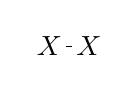
\begin{tikzpicture}[baseline={([yshift=-.5ex]current bounding box.center)}]
	\path (0,0) node (A) {$X$} ++ (0.5,0) node (B) {$X$};
	\draw (A) -- (B);
\end{tikzpicture}
\end{align}

We choose a particular 1-element set $\{*\}$ that acts as the identity in the sense that $\{*\}\times A\cong A\times \{*\} \cong A$ for any set $A$. The erase map $\text{del}_X:X\kto \{*\}$ defined by $(\text{del}_X)(*|x) = 1$ is a Markov kernel that ``discards the input''. It is drawn as a fuse:

\begin{align}
	\text{del}_X&:=\begin{tikzpicture}[baseline={([yshift=-.5ex]current bounding box.center)}]
	\path (0,0) ++ (1,0) node (B) {$X$};
	\draw[-{Rays[n=8]}] (A) -- (B);
\end{tikzpicture}
\end{align}

The copy map $\text{copy}_X:X\kto X\times X$ defined by $(\text{copy}_X)(x',x''|x)=\llbracket x=x' \rrbracket \llbracket x=x'' \rrbracket$ is a Markov kernel that makes two identical copies of the input. It is drawn as a fork:

\begin{align}
	\text{copy}_X&:=\begin{tikzpicture}[baseline={([yshift=-.5ex]current bounding box.center)}]
	\path (0,0) node (A) {$X$} 
	++ (0.5,0) node[copymap] (copy0) {}
	++ (0.5,0.15) node (B) {$X$}
	+ (0,-0.3) node (C) {$X$};
	\draw (A) -- (copy0) to [out=45,in=180] (B) (copy0) to [out=-45, in=180] (C);
\end{tikzpicture}
\end{align}

The swap map $\text{swap}_{X,Y}:X\times Y\kto Y\times X$ defined by $(\text{swap}_{X,Y})(y',x'|x,y)=\llbracket x=x' \rrbracket\llbracket y=y' \rrbracket$ swaps two inputs, and is represented by crossing wires:

\begin{align}
	\text{swap}_X &:=  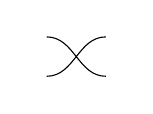
\begin{tikzpicture}[baseline={([yshift=-.5ex]current bounding box.center)}]
		\path (0,0) node (A) {} 
		+ (0,-0.5) node (B) {}
		++ (1,0) node (C) {}
		+ (0,-0.5) node (D) {};
		\draw (A) to [out=0,in=180] (D) (B) to [out=0, in=180] (C);
	\end{tikzpicture}
\end{align}

Because we anticipate that the graphical notation will be unfamiliar, we will include some examples in the next section.

\subsubsection{Examples}

When translating string diagram notation to integral notation, a number of identities can speed up the process.

For arbitrary $\kernel{K}:X\times Y\to Z$, $\kernel{L}:W\to Y$

\begin{align}
 [(\text{id}_X\otimes \kernel{L})\kernel{K}](A|x,w) &= \int_{Y}\int_X   \kernel{K}(z|x',y')\kernel{L}(dy'|w)\text{id}_X(dx'|x)\\
										   &= \int_Y  \kernel{K}(z|x,y') \kernel{L}(dy'|w)
\end{align}

That is, an identity map passes its input to the next kernel in the product. 

For arbitrary $\kernel{K}: X\times Y\times Y\to Z$ (where we apply the above shorthand in the first line):

\begin{align}
 [(\text{id}_X\otimes \text{copy}_Y)\kernel{K}](A|x,y) &= \int_Y\int_Y \kernel{K}(A|x,y',y'') \text{copy}_Y(dy'\times dy''|y)\\
										   &= \kernel{K}(A|x,y,y)
\end{align}

That is, the copy map passes along two copies of its input to the next kernel in the product. 

For a collection of kernels $\kernel{K}^n:Y^n\to Z$, $n\in[n]$, define $(y)^{n}=(y|i\in[n])$ and:

\begin{align}
	\text{copy}^n_Y &:= \begin{cases}
	\text{copy}^{n-1}_Y(\text{id}_{Y^{n-2}}\otimes \text{copy}_Y) & n>2\\
	\text{copy}_Y & n=2
	\end{cases}\\
	(\text{copy}^2_Y\kernel{K}^2)(z|y) &= \kernel{K}^2(z|y,y)\\
\end{align}

Suppose for induction
\begin{align}
(\text{copy}^{n-1}_Y\kernel{K}^{n-1})(z|y) &= \kernel{K}^{n-1}(z|(y)^{n-1})
\end{align}

then
\begin{align}
(\text{copy}^n_Y\kernel{K}^n)(z|y) &= (\text{copy}^{n-1}_Y(\text{id}_{Y^{n-2}}\otimes \text{copy}_Y)\kernel{K}^n)(z|y)\\
									 &= \sum_{y'\in Y^{n-1}}(\text{id}_{Y^{n-2}}\otimes \text{copy}_Y)(\mathbf{y}'|(y)^{n-1})\kernel{K}^n(z|\mathbf{y}')\\
									 &= \kernel{K}^n(z|(y)^n)
\end{align}

That is, we can define the $n$-fold copy map that passes along $n$ copies of its input to the next kernel in the product.

\subsubsection{Example: comb insertion}

The following examples illustrate 2-combs and the insertion operation, both of which we will define later. As an example in translating diagrams, we show how the diagrams for a 2-comb and 2-comb with an inserted Markov kernel can be translated to integral notation.

Consider the Markov kernels $\kernel{K}:W\kto X$, $\kernel{L}:X\times W\times Y\kto Z$ and the 2-comb $\kernel{M}:W\times Y\kto X\times Z$ defined as

\begin{align}
	\kernel{M} = \tikzfig{2_comb}\label{eq:2comb_M}
\end{align}

Following the rules above, we can translate this to ordinary notation by first breaking it down into products and tensor products, and then evaluating these products

\begin{align}
	\kernel{M}(A\times B|w,y) = [&(\text{copy}_W\otimes \text{id}_Y)(\kernel{K}\otimes \text{id}_{W\times Y})\\
	&(\text{copy}_X\otimes \text{id}_{W\times Y})(\text{id}_X\otimes\kernel{L})](A\times B|w,y)\\
						= [&(\kernel{K}\otimes \text{id}_{W\times Y})(\text{copy}_X\otimes \text{id}_{W\times Y})\\
						&(\text{id}_X\otimes\kernel{L})](A\times B|w,w,y)\\
						= \;&\int_{X}  (\text{id}_X\otimes\kernel{L})(A\times B|x',w,y) \kernel{K} (dx'|w)
						](y,z|y',x)\\
						= \;&\int_X \text{id}_X(A|x') \kernel{L}(B|x',w,y)\kernel{K}(dx'|w)\\
						= \;&\int_A \kernel{L}(B|x',w,y)\kernel{K}(dx'|w)
\end{align}

If we are given additionally $\kernel{J}:X\times W\kto Y$, we can define a new Markov kernel $\kernel{N}:W\kto Z$ given by ``inserting'' $\kernel{J}$ into $\kernel{M}$:

\begin{align}
	\kernel{N} = \tikzfig{2comb_inserted_anon}\label{eq:2comb_winsert}
\end{align}


We can translate Equation \ref{eq:2comb_winsert} to

\begin{align}
	\kernel{N}(A\times B\times C|w) = &[\text{copy}_W(\kernel{K}\text{copy}^3_Y\otimes \text{id}_W)\\
	&(\text{id}_Y\otimes\kernel{J}\otimes \text{id}_Y)(\text{id}_Y \otimes \text{copy}_X\otimes \text{id}_Y)\\
	&(\kernel{L}\otimes \text{id}_X\otimes \text{id}_Y)] (A\times B\times C|w)\\
					= &[(\kernel{K}\text{copy}^3_Y\otimes \text{id}_W)(\text{id}_Y\otimes\kernel{J}\otimes \text{id}_Y)\\
					&(\text{id}_Y \otimes \text{copy}_X\otimes \text{id}_Y)\\
					&(\kernel{L}\otimes \text{id}_X\otimes \text{id}_Y)] (A\times B\times C|w,w)\\
					= &\int_X\int_Y\kernel{L}(C|x',w,y') \text{id}_X(A|x') \text{id}_Y(B|y') \kernel{J}(dy'|x',w)\kernel{K}(dx'|w)\\
					= &\int_A\int_B\kernel{L}(C|x',w,y') \kernel{J}(dy'|x',w)\kernel{K}(dx'|w)
\end{align}

\subsection{Semantics of observed and unobserved variables}\label{sec:variables}

We are interested in constructing \emph{probabilistic models} which explain some part of the world. In a model, variables play the role of ``pointing to the parts of the world the model is explaining''. Both observed an unobserved variables play important roles in causal modelling and we think it is worth clarifying what variables of either type refer to. Our approach is a standard one: a probabilistic model is associated with an experiment or measurement procedure that yields values in a well-defined set. Observable variables are obtained by applying well-defined functions to the result of this total measurement. We use a richer fundamental probability set that includes ``unobserved variables'' that are formally treated the same way as observed variables, but aren't associated with any real-world counterparts.

Consider Newton's second law in the form $\proc{F}=\proc{MA}$ as a simple example of a model that relates ``variables'' $\proc{F}$, $\proc{M}$ and $\proc{A}$. As \citet{feynman_feynman_1979} noted, this law is incomplete -- in order to understand it, we must bring some pre-existing understanding of force, mass and acceleration as independent things. Furthermore, the nature of this knowledge is somewhat perculiar. Acknowledging that physicists happen to know a great deal about forces on an object, it remains true that in order to actually say what the net force on a real object is, even a highly knowledgeable physicist will still have to go and do some measurements, and the result of such measurements will be a vector representing the net forces on that object.

This suggests that we can think about ``force'' $\proc{F}$ (or mass or acceleration) as a kind of procedure that we apply to a particular real world object and which returns a mathematical object (in this case, a vector). We will call $\proc{F}$ a \emph{procedure}. Our view of $\proc{F}$ is akin to \citet{menger_random_2003}'s notion of variables as ``consistent classes of quantities'' that consist of pairing between real-world objects and quantities of some type. Force $\proc{F}$ itself is not a well-defined mathematical thing, as measurement procedures are not mathematically well-defined. At the same time, the set of values it may yield \emph{are} well-defined mathematical things. No actual procedure can be guaranteed to return elements of a mathematical set known in advance -- anything can fail -- but we assume that we can study procedures reliable enough that we don't lose much by making this assumption.

\begin{definition}[Measurement procedure]
A \emph{measurement procedure} is a procedure that involves interacting with the real world somehow and delivering an element of a mathematical set as a result. The set of possible values is known prior to the measurement taking place, but the value that it will yield is not known. A procedure is given the font $\proc{B}$, we say it takes values in $X$ and $\proc{B}\yields x$ is the proposition that the the procedure $\proc{B}$ will yield the value $x\in X$. $\proc{B}\yields A$ for $A\subset X$ is the proposition $\lor_{x\in A} \proc{B}\yields x$. Two procedures $\proc{B}$ and $\proc{C}$ are the same if $\proc{B}\yields x\iff \proc{C}\yields x$ for all $x\in B$ (note that $\proc{B}$ and $\proc{C}$ could involve different actions in the real world).
\end{definition}

Measurement procedures are like functions without well-defined domains. We can compose measurement procedures with functions to produce new measurement procedures.

\begin{definition}[Composition of functions with procedures]
Given a procedure $\proc{B}$ that takes values in some set $B$, and a function $f:B\to C$, define the ``composition'' $f\circ \proc{B}$ to be any procedure $\proc{C}$ that yields $f(x)$ whenever $\proc{B}$ yields $x$. We can construct such a procedure by describing the steps: first, do $\proc{B}$ and secondly, apply $f$ to the value yielded by $\proc{B}$.
\end{definition}

For example, $\proc{MA}$ is the composition of $h:(x,y)\mapsto xy$ with the procedure $(\proc{M},\proc{A})$ that yields the mass and acceleration of the same object. Measurement procedure composition is associative:

\begin{align}
	(g\circ f)\circ\proc{B}\text{ yields } x &\iff B\text{ yields } (g\circ f)^{-1}(x) \\
	&\iff B\text{ yields } f^{-1}(g^{-1}(x))\\
	&\iff f\circ B \text{ yields } g^{-1}(x)\\
	&\iff g\circ(f\circ B)\text{ yields } x
\end{align}


One might whether there is also some kind of ``append'' operation that takes a standalone $\proc{M}$ and a standalone $\proc{A}$ and returns a procedure $(\proc{M},\proc{A})$. Unlike function composition, this would be an operation that acts on two procedures rather than a procedure and a function. Unlike composition, we can't easily reason about such an operation mathematically, because of the fact that measurment procedures have a foot in the real world. Our approach here is to suppose that there is some master measurement procedure $\proc{S}$ which takes values in $\Psi$ that handles all of the ``real world'' interaction relevant to our problem. Specifically, we assume that any measurement procedure of interest to our problem can be written as the composition $f\circ \proc{S}$ for some $f$.

For the model $\proc{F}=\proc{MA}$, for example, we could assume $\proc{F}=f\circ \proc{S}$ for some $f$ and $(\proc{M},\proc{A})=g\circ \proc{S}$ for some $g$. In this case, we can get $\proc{MA}=h\circ(\proc{M},\proc{A})=(h\circ g)\circ\proc{S}$. Note that each procedure is associated with a unique function with domain $\Psi$.

Thus far we have defined by $\Psi$ a ``fundamental probability set'' limited to observable variables -- which is to say, limited to variables that are associated with measurement procedures. Unobserved variables need not be associated with measurement procedures, and to accommodate these we use instead of $\Psi$ a richer fundamental probability set $\Omega$ which represents both observed and unobserved variables.

\begin{definition}[Fundamental probability set]
The fundamental probability set (or \emph{sample space}) $\Omega$ is a measurable set with $\sigma$-algebra $\sigalg{F}$.
\end{definition}

Observables are represented by a function $\RV{S}:\Omega\to \Psi$, and values of $\omega$ are related to propositions about measurement procedures via the criterion of \emph{consistency with observation}.

\begin{definition}[Consistency with observation]\label{def:observable}
An element $\omega\in \Omega$ is is \emph{consistent with observation} if the result yielded by $\proc{S}\yields \RV{S}(\omega)$
\end{definition}

Thus the procedure $\proc{S}$ restricts the observationally consistent elements of $\Omega$. If $\proc{S}$ yield the result $s$, then the consistent values of $\Omega$ will be $\RV{S}^{-1}(s)$. While two different sets of measurement outcomes $\Psi$ and $\Psi'$ entail a different mesurement procedures $\proc{S}$ and $\proc{S}'$, but different fundamental probability sets $\Omega$ and $\Omega'$ may be used to model a single procedure $\proc{S}$.

As far as we know, distinguishing variables from procedures is somewhat nonstandard, but we feel it is useful to distinguish the formal elements of our theory (variables) from the semi-formal elements (measurement procedures). Both variables and procedures are often discussed in statistical texts. For example, \citet{pearl_causality:_2009} offers the following two, purportedly equivalent, definitions of variables:
\begin{quote}
By a \emph{variable} we will mean an attribute, measurement or inquiry that may take on one of several possible outcomes, or values, from a specified domain. If we have beliefs (i.e., probabilities) attached to the possible values that a variable may attain, we will call that variable a random variable.
\end{quote}

\begin{quote}
This is a minor generalization of the textbook definition, according to which a random variable is a mapping from the fundamental probability set (e.g., the set of elementary events) to the real line. In our definition, the mapping is from the fundamental probability set to any set of objects called ``values,'' which may or may not be ordered.
\end{quote}

Our view is that the first definition is a definition of a procedure, while the second is a definition of a variable. Variables model procedures, but they are not the same thing. We can establish this by noting that, under our definition, every procedure of interest -- that is, all procedures that can be written $f\circ \proc{S}$ for some $f$ -- is modeled by a variable, but there may be variables defined on $\Omega$ that do not factorise through $\proc{S}$, and these variables do not model procedures.

\subsection{Events}

To recap, we have a procedure $\proc{S}$ yielding values in $\Psi$ that measures everything we are interested in, a fundamental probability set $\Omega$ and a function $\RV{S}$ that models $\proc{S}$ in the sense of Definition \ref{def:observable}. We assume also that $\Psi$ has a $\sigma$-algebra $\sigalg{E}$ (this may be the power set of $\Psi$, as measurement procedures are typically limited to finite precision). $\Omega$ is equipped with a $\sigma$-algebra $\sigalg{F}$ such that $\sigma(\RV{S})\subset \sigalg{F}$. If a procedure $\proc{X}=f\circ \RV{S}$ then we define $\RV{X}:\Omega\to X$ by $\RV{X}:=f\circ\RV{S}$.

If a particular procedure $\proc{X}=f\circ \proc{S}$ eventually yields a value $x$, then the values of $\Omega$ consistent with observation must be a subset of $\RV{X}^{-1}(x)$. We define an \emph{event} $\RV{X}\yields x:\equiv \RV{X}^{-1}(x)$, which we read ``the event that $\RV{X}$ yields x''. An event $\RV{X}\yields x$ occurs if the consistent values of $\Omega$ are a subset of $\RV{X}\yields x$, thus ``the event that $\RV{X}$ yields x occurs$\equiv \proc{X}$ yields $x$''. The definition of events applies to all types of variables, not just observables, but we only provide an interpretation of events ``occurring'' when the variable $\RV{X}$ is associated with some $\proc{X}$.

For measurable $A\in \sigalg{X}$, $\RV{X}\yields A=\bigcup_{x\in A} \RV{X}\yields x$. 

Given $\RV{Y}:\Omega\to X$, we can define a sequence of variables: $(\RV{X},\RV{Y}):=\omega\mapsto (\RV{X}(\omega),\RV{Y}(\omega))$. $(\RV{X},\RV{Y})$ has the property that $(\RV{X},\RV{Y})\yields (x,y)= \RV{X}\yields x\cap \RV{Y}\yields y$, which supports the interpretation of $(\RV{X},\RV{Y})$ as the values yielded by $\RV{X}$ and $\RV{Y}$ together.

It is common to use the symbol $=$ instead of $\bowtie$, but we want to avoid this because $\RV{Y}=y$ already has a meaning, namely that $\RV{Y}$ is a constant function everywhere equal to $y$. 

\subsection{Probabilistic models for causal inference}

The fundamental probability set $(\Omega,\sigalg{F})$ along with our collection of variables is a ``model skeleton'' -- it tells us what kind of data we might see. The process $\proc{S}$ which tells us which part of the world we're interested in is related to the model $\Omega$ and the observable variables by the criterion of \emph{consistency with observation}. The kind of problem we are mainly interested in here is one where we make use of data to help make decisions under uncertainty. Probabilistic models have a long history of being used for this purpose, and our interest here is in constructing probabilistic models that can be attached to our variable ``skeleton''. 

Given a model skeleton, a common approach to attaching a probabilistic model involves defining a base measure $\mu$ on $\Omega$ which yields a probability space $(\Omega,\sigalg{F},\mu)$. For causal inference, we need a to generalise this approach, because we need to handle \emph{gaps} in our model. \citet{hajek_what_2003} defines \emph{probability gaps} as propositions that do not have a probability assigned to them. Our view of probability gaps is slightly different -- in this work, a model with probability gaps as one that is missing some key parts or ``inserts''. If we complete such a model with an appropriate insert, we get a standard probability model.

Probability gap models are particularly useful in for decision making. When I have a number of different options I could choose, I need a model that tells me what is likely to happen for each choice I could make. Thus I need a model that can take a provisional choice as an argument and return a probability model representing the results of this choice; in other words, the choices I may make are \emph{probability gaps}.

We impose some additional conditions on probability gap models. In particular, a probability gap model imposes some requirements on the final probability distributions of interest; that is, it defines a \emph{probability set}, which is a subset of probability models on $(\Omega,\sigalg{F})$. Probability gaps are sets of alternative requirements we can impose on the final distributions of interest; that is, probability gaps are sets of probability sets. We call the elements of a probability gap a \emph{probability insert}. The logic of a probability gap model is thus: we take a probability set representing the \emph{model}, and choose one probability insert from several alternatives that together make a probability gap; the final model of interest is the probability set obtained by intersecting the model with the insert.

This scheme raises the possibility that the model, the insert, or the intersection may be empty if we are not careful. We define the notion of \emph{validity} and show that it is sufficient that the probability model and the probability insert are valid for the intersection to be non-empty.

\subsection{Probability sets}

\todo[inline]{Note for proofreading}
I've been adding decorations $\prob{P}$, $\prob{P}_{\{\}}$ and $\prob{P}_{\square}$ to denote probability models, probability sets and probability gap models respectively, but I'm not close to adding them everywhere they are needed yet.
\todo[inline]{end note}

A probability set is a set of gap model is a function that maps ``inserts'' to probability models. We think of the set of inserts as different ways we can fill the probability gap. The particular kinds of inserts we want to consider here are marginal probabilities and conditional probabilities.

\begin{definition}[Probability space]
A probability space is a triple $(\mu,\Omega,\sigalg{F})$, where $\mu$ is a base measure on $\sigalg{F}$ which we here take to be $\mathscr{P}(\Omega)$.
\end{definition}

\begin{definition}[Probability set]
A probability set $\prob{P}_{\{\}}$ on $(\Omega,\sigalg{F})$ is a collection of probability measures on $(\Omega,\sigalg{F})$. In other words it is a subset of $\mathscr{P}(\Delta(\Omega))$.
\end{definition}

\begin{definition}[Probability gap model]
Given a fundamental probability set $\Omega$ and a set of probability sets $A$, a probability gap model $\prob{P}_\square:A\to \mathscr{P}(\Delta(\Omega))$ is a function that sends an element of $A$ to a probability set on $\Omega$.
\end{definition}

We will make a substantial simplifying assumption: all sets, including the fundamental probability set $\Omega$ and any set of values a variable takes, are discrete sets. That is, they are at most countably infinite and the $\sigma$-algebra of measurable sets is the power set. Because we are working with discrete sets we will by convention call probability measures on set elements: $\prob{P}^{\RV{X}}(x):=\prob{P}^{\RV{X}}(\{x\})$.

Probability spaces along with random variables can be used to define \emph{marginal probability distributions} of those random variables.

\begin{definition}[Marginal distribution with respect to a probability space]\label{def:pushforward}
Given a probability space $(\mu,\Omega)$ and a random variable $\RV{X}:\Omega\to X$, we can define the \emph{marginal distribution} of $\RV{X}$ with respect to $\mu$, $\mu^{\RV{X}}:\sigalg{X}\to [0,1]$ of $\RV{X}$ by $\mu^{\RV{X}}(x):=\mu(\RV{X}\yields x)$ for any $x\in X$. Equivalently, if we define the Markov kernel $\kernel{F}_{\RV{X}}:\Omega\kto X$ associated with the function $\RV{X}$ by $\kernel{F}_{\RV{X}}(x|\omega)=\llbracket \RV{X}(\omega)=x\rrbracket$, then
\begin{align}
	\mu^{\RV{X}} = \mu\kernel{F}_{\RV{X}}
\end{align}
\end{definition}

A $\RV{Y}|\RV{X}$-\emph{conditional probability} is ``the probability of $\RV{Y}$ given $\RV{X}$ relative to $\mu$''. It is a Markov kernel that maps the marginal distribution of $\RV{X}$ to the marginal distribution of the sequence $(\RV{X},\RV{Y})$.

\begin{definition}[Conditional probability with respect to a probability space]\label{def:disint}
Given a probability space $(\mu,\Omega)$ and random variables $\RV{X}:\Omega\to X$, $\RV{Y}:\Omega\to Y$, the disintegration $\mu^{\RV{Y}|\RV{X}}:X\kto Y$ is any Markov kernel such that
\begin{align}
	\mu^{\RV{X}}(x)\mu^{\RV{Y}|\RV{X}}(y|x)&= \mu^{\RV{XY}}(x,y) &\forall x\in X, y\in Y\\
	&\iff\\
	\tikzfig{disint_def} &= \mu^{\RV{XY}}
\end{align}
\end{definition}

Given a probability set $\prob{P}_{\{\}}$, we define marginal and conditional probabilities as probability measures and Markov kernels that satisfy Definitions \ref{def:pushforward} and \ref{def:disint} respectively for \emph{all} base measures in $\prob{P}_{\{\}}$. 

Even though there are generally multiple Markov kernels that satisfy the properties of a conditional probability with respect to a probability set, this definition ensures that any choice will map the same marginal distribution to the same joint distribution \emph{no matter which base measure we choose}.

\begin{definition}[Marginal probability with respect to a probability set]
Given a fundamental probability set $\Omega$ a variable $\RV{X}:\Omega\to X$ and a probability set $\prob{P}_{\{\}}$, the marginal distribution $\prob{P}_{\{\}}^{\RV{X}}=\prob{P}_a^{\RV{X}}$ for any $\prob{P}_a\in\prob{P}_{\{\}}$ if a distribution satisfying this condition exists. Otherwise, it is undefined.
\end{definition}

\begin{definition}[Conditional probability with respect to a probability set]
Given a fundamental probability set $\Omega$ variables $\RV{X}:\Omega\to X$ and $\RV{Y}:\Omega\to Y$ and a probability set $\prob{P}_{\{\}}$, $\prob{P}_{\{\}}^{\RV{Y}|\RV{X}}$ is any Markov kernel $X\kto Y$ such that for all $\prob{P}_a\in \prob{P}_{\{\}}$:
\begin{align}
	\prob{P}_a^{\RV{X}}(x)\prob{P}^{\RV{Y}|\RV{X}}(y|x)&= \prob{P}_a^{\RV{XY}}(x,y) &\forall x\in X, y\in Y
\end{align}
If no such Markov kernel exists, $\prob{P}_{\{\}}^{\RV{Y}|\RV{X}}$ is undefined.
\end{definition}

Given a conditional probability with respect to a probability gap model, we can find other conditional probabilities by ``pushing it forward''.

\begin{lemma}[Equivalence of pushforward definitions]\label{lem:prod_pushf}
Given a probability space $\kernel{M}:W\to \Omega$ and $\RV{X}:\Omega\to X$, define $\kernel{K}^{\RV{X}|\RV{W}}:W\kto X$ by $\kernel{K}^{\RV{X}|\RV{W}}(x|w):=\kernel{M}(\RV{X}\yields x|w)$ for any $x\in X$m $w\in W$ and $\kernel{L}^{\RV{X}}:W\kto X$ by
\begin{align}
	\kernel{L}^{\RV{X}|\RV{W}} = \kernel{M}\kernel{F}_{\RV{X}}
\end{align}
Then
\begin{align}
\kernel{L}^{\RV{X}|\RV{W}} =\kernel{K}^{\RV{X}|\RV{W}}
\end{align}
\end{lemma}

\begin{proof}
For any $x\in X$, $w\in W$
\begin{align}
	\kernel{L}^{\RV{X}|\RV{W}}(x|w) &= \sum_{\omega\in \Omega} \llbracket x=\RV{X}(\omega)\rrbracket \kernel{M}(\omega|w)\\
									&= \sum_{\omega\in \RV{X}^{-1}(x)} \kernel{M}(\omega|w)\\
									&= \kernel{M}(\RV{X}\yields x|w)\\
									&= \kernel{K}^{\RV{X}|\RV{W}}(x|w)
\end{align}
\end{proof}

\begin{theorem}[Recursive pushforward]\label{th:recurs_pushf}
Suppose we have a fundamental probability set $\Omega$ variables $\RV{X}:\Omega\to X$ and $\RV{Y}:\Omega\to Y$, $\RV{Z}:\Omega\to Z$ and a probability set $\prob{P}_{\{\}}$ such that $\prob{P}_{\{\}}^{\RV{X}|\RV{Y}}$ is a $\RV{Y}|\RV{X}$ conditional probability of $\prob{P}_{\{\}}$ and $\RV{Z}=f\circ \RV{Y}$ for some $f:Y\to Z$. Then there exists a $\RV{Z}|\RV{X}$ conditional probability of $\prob{P}_{\{\}}$ given by $\prob{P}_{\{\}}^{\RV{Z}|\RV{X}}=\prob{P}_{\{\}}^{\RV{Y}|\RV{X}}\kernel{F}_{f}$.
\end{theorem}

\begin{proof}
For any $\prob{P}_a\in \prob{P}_{\{\}}$, $x,z$
\begin{align}
\prob{P}_a^{\RV{X}}(x)\prob{P}_a^{\RV{Z}|\RV{X}}(z|x) &= \prob{P}_a(\RV{X}^{-1}(x)\cap\RV{Z}^{-1}(z))\\
					   &= \prob{P}_a(\RV{X}^{-1}(x)\cap\RV{Y}^{-1}(f^{-1}(z)))\\
					   &= \prob{P}_a^{\RV{X},\RV{Y}}(\{x\}\times f^{-1}(z))\\
					   &= \prob{P}_a^{\RV{X}}(x)\prob{P}_a^{\RV{Y}|\RV{X}}(f^{-1}(z)|x)
\end{align}
\end{proof}

We also generalise the notion of almost sure equality with respect to a probability set to mean almost sure equality with respect to every base measure in the set

\begin{definition}[Almost sure equality]
Two functions $f:\Omega\to X$ and $g:\Omega\to Y$ are almost surely equal with respect to a probability set $\prob{P}_{\{\}}$ if they are almost surely equal with respect to every base measure $\prob{P}\in \prob{P}_{\{\}}$.
\end{definition}

% \begin{theorem}[Disintegrations are conditional probabilities]
% Suppose we have a fundamental probability set $\Omega$ variables $\RV{W}:\Omega\to W$, $\RV{X}:\Omega\to X$, $\RV{Y}:\Omega\to Y$ and $\RV{Z}:\Omega\to Z$ and a probability set $\prob{P}_{\{\}}$ such that $\prob{P}_{\{\}}^{\RV{X}|\RV{Y}}$ is a $\RV{Y}|\RV{X}$ conditional probability and there is some $\kernel{K}^{\RV{$
% \end{theorem}

% Given a conditional probability with respect to a probability gap model, we can also find additional conditional probabilities by disintegrating the original conditional probability.

% \begin{lemma}[Recursive disintegration]
% Suppose we have a fundamental probability set $\Omega$, variables $\RV{W}:\Omega\to W$, $\RV{X}:\Omega\to X$ and $\RV{Y}:\Omega\to Y$, $\RV{Z}:\Omega\to Z$ and a probability set $\prob{P}_{\{\}}$ such that $\prob{P}_{\{\}}^{\RV{X}|\RV{Y}}$ is a $\RV{Y}|\RV{X}$ conditional probability. Define $\prob{Q}_{\{\}}$ as the largest probability set such that $\prob{Q}_{\{\}}^{\RV{Y}|\RV{X}}=\prob{P}_{\{\}}^{\RV{Y}|\RV{X}}$. Then if $\prob{Q}_{\{\}}^{\RV{Z}|\RV{W}}$ is a $\RV{Z}|\RV{W}$ conditional probability of $\prob{Q}_{\{\}}$, it is also a $\RV{Z}|\RV{W}$ conditional probability of $\prob{P}_{\{\}}$.
% \end{lemma}

% \begin{proof}
% $\prob{Q}_{\{\}}\supset \prob{P}_{\{\}}$, so any conditional probability of $\prob{Q}_{\{\}}$ is also a conditional probability of $\prob{P}_{\{\}}$.
% \end{proof}

\subsection{Probability sets defined by marginal and conditional probabilities}

In the previous section we defined marginal and conditional probabilities for probability sets. We can define probability sets by marginal or conditional probabilities as the set of all probability models that share those marginals or conditionals.

Not all probability measures $\prob{Q}^{\RV{X}}$ on $X$ define nonempty sets of probability measures on $\Omega$. Consider, for example, $\RV{X}=(\RV{Y},\RV{Y})$ for some $\RV{Y}:\Omega\to Y$ and any measure $\prob{Q}^{\RV{YY}}$ that assigns nonzero probability to the event $(\RV{Y},\RV{Y})\yields (y,y')$ for $y\neq y'$. Then there is no base measure that pushes forward to $\prob{P}^{\RV{YY}}$. A \emph{valid candidate distribution} is a distribution associated with a particular variable that defines a nonempty set of base measures on $\Omega$.

\begin{definition}[Valid canditate distribution]\label{def:valid_dist}
A valid $\RV{X}$-probability distribution $\prob{P}^{\RV{X}}$ is any probability mesure on $\Delta(X)$ such that $\RV{X}^{-1}(A)=\emptyset\implies \prob{P}^{\RV{X}}(A) = 0$ for all $A\in\sigalg{X}$.
\end{definition}


\begin{theorem}[Validity]\label{th:completion}
Given $(\Omega,\sigalg{F})$, $\RV{X}:\Omega\to X$, $\kernel{J}\in \Delta(X)$ with $\Omega$ and $X$ standard measurable, there exists some $\mu\in \Delta(\Omega)$ such that $\mu^{\RV{X}}=\kernel{J}$ if and only if $\kernel{J}$ is a valid candidate distribution.
\end{theorem}

\begin{proof}
If:
This is a Theorem 2.5 of \citet{ershov_extension_1975}.
Only if:
This is also found in \citet{ershov_extension_1975}, but is simple enough to reproduce here. Suppose $\kernel{J}$ is not a valid probability distribution. Then there is some $x\in X$ such that $\RV{X}\yields x = \emptyset$ but $\kernel{J}(x)>0$. Then
\begin{align}
	\mu^{\RV{X}}(x) &= \mu (\RV{X}\yields x)\\
	&= \sum_{x'\in X} \kernel{J}(x') \kernel{K}(\RV{X}\yields x|x')\\
	&= 0\\
	&\neq \kernel{J}(x)
\end{align}
\end{proof}

\begin{definition}[Valid candidate conditional]\label{def:valid_conditional_prob}
Given $(\Omega,\sigalg{F})$, $\RV{X}:\Omega\to X$, $\RV{Y}:\Omega\to Y$ a \emph{valid $\RV{Y}|\RV{X}$ conditional probability} $\prob{P}^{\RV{Y}|\RV{X}}$ is a Markov kernel $X\kto Y$ such that it assigns probability 0 to contradictions:
\begin{align}
	\forall B\in \sigalg{Y}, x\in \sigalg{X}: (\RV{X},\RV{Y})\yields \{x\}\times B = \emptyset \implies \left(\prob{P}^{\RV{Y}|\RV{X}}(A|x) = 0\right) \lor \left(\RV{X}\yields \{x\} = \emptyset\right)
\end{align}
\end{definition}

The definition of conditional probability (Definition \ref{def:disint}) allows in some cases for conditional probabilities that are not valid candidate conditionals. In Theorem \ref{th:valid_disint} we prove that it is always possible to choose a version of a conditional probability that is also a valid candidate conditional. See also \citet{hajek_what_2003} for an argument that conditional probabilities should always satisfy the property of being valid candidate conditionals.

The particular property we show for valid candidate conditionals is that if we combine them with other valid candidate conditionals via the operation $\odot$ (Definition \ref{def:copyproduct}) then we are left with a valid candidate conditional (Theorem \ref{th:valid_conditional_probability}). This reduces to a valid candidate distribution in the case of conditioning on the trivial variable $*$ (Lemma \ref{th:valid_agree}). Because $\odot$ leaves us with a subset of the intersection of the probability sets defined by the two inputs (Theorem \ref{th:intersection}), this also shows that valid candidate conditionals define non-empty probability sets.

Therefore, as long as we limit ourselves to valid candidate conditionals, we can use them to represent probability sets and intersect the sets using $\odot$ and we are guaranteed not to end up with empty probability sets.

\begin{definition}[Copy-product]\label{def:copyproduct}
Given two Markov kernels $\prob{K}:X\kto Y$ and $\prob{L}:Y\times X\kto Z$, define the copy-product $\prob{K}\odot\prob{L}:X\to Y\times Z$ as
\begin{align}
	\prob{K}\odot\prob{L}:&= \text{copy}_X(\prob{K}\otimes \text{id}_X)(\text{copy}_Y\otimes\text{id}_X )(\text{id}_Y \otimes \prob{L})\\
							&= \tikzfig{copy_product}\\
							&\iff\\
	(\prob{K}\odot\prob{L})(A\times B|x) &= \int_B \prob{L}(A|y,x)\prob{K}(dy|x)
\end{align}
\end{definition}

\begin{theorem}[Copy-product is an intersection of probability sets]\label{th:intersection}
Given $\Omega$, $\RV{X}$, $\RV{Y}$, $\RV{Z}$ all standard measurable, and valid candidate conditionals $\prob{P}_{\{\}}^{\RV{Y}|\RV{X}}$ and $\prob{Q}_{\{\}}^{\RV{Z}|\RV{YX}}$ with $\prob{P}_{\{\}}$ the largest probability set with conditional $\prob{P}_{\{\}}^{\RV{Y}|\RV{X}}$ and $\prob{Q}_{\{\}}$ the largest probability set with conditional $\prob{Q}_{\{\}}^{\RV{Z}|\RV{YX}}$, then the largest probability set $\prob{R}_{\{\}}$ with conditional $\prob{R}_{\{\}}^{\RV{YZ}|\RV{X}}=\prob{P}_{\{\}}^{\RV{Y}|\RV{X}}\odot \prob{Q}_{\{\}}^{\RV{Z}|\RV{YX}}$ is equal to $\prob{R}_{\{\}}=\prob{P}_{\{\}}\cap\prob{Q}_{\{\}}$.
\end{theorem}

\todo[inline]{Make sure this works for a.s. equality}

\begin{proof}
By Theorem \ref{th:recurs_pushf}, $\prob{R}_{\{\}}^{\RV{Y}|\RV{X}}=\prob{P}_{\{\}}^{\RV{Y}|\RV{X}}$ so $\prob{R}_{\{\}}\subset\prob{P}_{\{\}}$. Furthermore by construction $\prob{R}_{\{\}}^{\RV{Z}|\RV{YX}}=\prob{Q}_{\{\}}^{\RV{Z}|\RV{YX}}$ so $\prob{R}_{\{\}}\subset \prob{P}_{\{\}}\cap\prob{Q}_{\{\}}$.

Suppose there's an element $\prob{S}$ of $\prob{P}_{\{\}}\cap\prob{Q}_{\{\}}$ not in $\prob{R}_{\{\}}$. Then $\prob{S}^{\RV{YZ}|\RV{X}}\neq \prob{R}_{\{\}}^{\RV{YZ}|\RV{X}}$. But by assumption $\prob{S}^{\RV{Z}|\RV{YX}} = \prob{R}_{\{\}}^{\RV{Z}|\RV{YX}}$ and $\prob{S}^{\RV{Y}|\RV{X}} = \prob{R}_{\{\}}^{\RV{Y}|\RV{X}}$. But then $\prob{S}^{\RV{YX}|\RV{X}} = \prob{R}_{\{\}}^{\RV{Y}|\RV{X}} \odot \prob{R}_{\{\}}^{\RV{Z}|\RV{YX}} = \prob{R}_{\{\}}^{\RV{YZ}|\RV{X}}$, contradiction.
\end{proof}

\begin{lemma}[Equivalence of validity definitions]\label{th:valid_agree}
Given $\RV{X}:\Omega\to X$, with $\Omega$ and $X$ standard measurable, a probability measure $\prob{P}^{\RV{X}}\in \Delta(X)$ is valid if and only if the conditional $\prob{P}^{\RV{X}|*}:=*\mapsto \prob{P}^{\RV{X}}$ is valid.
\end{lemma}

\begin{proof}
$*\yields *=\Omega$ necessarily. Thus validity of $\prob{P}^{\RV{X}|*}$ means 

\begin{align}
	\forall A\in \sigalg{X}: \RV{X}\yields A=\emptyset \implies \prob{P}^{\RV{X}|*}(A|*)&=0
\end{align}

But $\prob{P}^{\RV{X}|*}(A|*)=\prob{P}^{\RV{X}}(A)$ by definition, so this is equivalent to

\begin{align}
	\forall A\in \sigalg{X}: \RV{X}\yields A=\emptyset \implies \prob{P}^{\RV{X}}(A)&=0
\end{align}
\end{proof}


\begin{lemma}[Copy-product of valid candidate conditionals is valid]\label{lem:valid_extendability}
Given $(\Omega,\sigalg{F})$, $\RV{X}:\Omega\to X$, $\RV{Y}:\Omega\to Y$, $\RV{Z}:\Omega\to Z$ (all spaces standard measurable) and any valid candidate conditional $\prob{P}^{\RV{Y}|\RV{X}}$ and $\prob{Q}^{\RV{Z}|\RV{Y}\RV{X}}$, $ \prob{P}^{\RV{Y}|\RV{X}}\odot \prob{Q}^{\RV{Z}|\RV{Y}\RV{X}}$ is also a valid candidate conditional.
\end{lemma}

\begin{proof}
Let $\prob{R}^{\RV{YZ}|\RV{X}}:=\prob{P}^{\RV{Y}|\RV{X}}\odot \prob{Q}^{\RV{Z}|\RV{Y}\RV{X}}$.

We only need to check validity for each $x\in \RV{X}(\Omega)$, as it is automatically satisfied for other values of $\RV{X}$.

For all $x\in \RV{X}(\Omega)$, $B\in \sigalg{Y}$ such that $\RV{X}\yields \{x\}\cap\RV{Y}\yields B=\emptyset$, $\prob{P}^{\RV{Y}|\RV{X}}(B|x)=0$ by validity. Thus for arbitrary $C\in \sigalg{Z}$
\begin{align}
	\prob{R}^{\RV{YZ}|\RV{X}}(B\times C|x) &= \int_B \prob{Q}^{\RV{Z}|\RV{YX}}(C|y,x)\prob{P}^{\RV{Y}|\RV{X}}(dy|x)\\
								  &\leq \prob{P}^{\RV{Y}|\RV{X}}(B|x)\\
								  &=0
\end{align}

For all $\{x\}\times B$such that $\RV{X}\yields \{x\}\cap\RV{Y}\yields B\neq \emptyset$ and $C\in \sigalg{Z}$ such that $(\RV{X},\RV{Y},\RV{Z})\yields \{x\}\times B\times C=\emptyset$, $\prob{Q}^{\RV{Z}|\RV{YX}}(C|y,x)=0$ for all $y\in B$ by validity. Thus:
\begin{align}
	\prob{R}^{\RV{YZ}|\RV{X}}(B\times C|x) &= \int_B \prob{Q}^{\RV{Z}|\RV{YX}}(C|y,x)\prob{P}^{\RV{Y}|\RV{X}}(dy|x)\\
								  			&=0
\end{align}
\end{proof}

\begin{corollary}[Valid candidate conditional is validly extendable to a valid candidate distribution]\label{corr:valid_extend_order1}
Given $\Omega$, $\RV{U}:\Omega\to U$, $\RV{W}:\Omega\to W$ and a valid candidate conditional $\prob{T}^{\RV{W}|\RV{U}}$, then for any valid candidate conditional $\prob{V}^{\RV{U}}$, $\prob{V}^{\RV{U}}\odot \prob{T}^{\RV{W}|\RV{U}}$ is a valid candidate probability.
\end{corollary}

\begin{proof}
Applying Lemma \ref{lem:valid_extendability} choosing $\RV{X}=*$, $\RV{Y}=\RV{U}$, $\RV{Z}=\RV{W}$ and $\prob{P}^{\RV{Y}|\RV{X}}=\prob{V}^{\RV{U}|*}$ and $\prob{Q}^{\RV{Z}|\RV{YX}}=\prob{T}^{\RV{W}|\RV{U*}}$ we have $\prob{R}^{WU|*}:=\prob{V}^{\RV{U}|*}\odot \prob{T}^{\RV{W}|\RV{U}*}$ is a valid conditional probability. Then $\prob{R}^{\RV{WU}}\cong \prob{R}^{\RV{WU}|*}$ is valid by Theorem \ref{th:valid_agree}.
\end{proof}

\begin{theorem}[Validity of conditional probabilities]\label{th:valid_conditional_probability}
Suppose we have $\Omega$, $\RV{X}:\Omega\to X$, $\RV{Y}:\Omega\to Y$, with $\Omega$, $X$, $Y$ discrete. A conditional $\prob{T}^{\RV{Y}|\RV{X}}$ is valid if and only if for all valid candidate distributions $\prob{V}^{\RV{X}}$, $\prob{V}^{\RV{X}}\odot \prob{T}^{\RV{Y}|\RV{X}}$ is also a valid candidate distribution.
\end{theorem}

\begin{proof}
If: this follows directly from Corollary \ref{corr:valid_extend_order1}.

Only if: suppose $\prob{T}^{\RV{Y}|\RV{X}}$ is invalid. Then there is some $x\in X$, $y\in Y$ such that $\RV{X}\yields(x)\neq \emptyset$, $(\RV{X},\RV{Y})\yields(x,y)=\emptyset$ and $\prob{T}^{\RV{Y}|\RV{X}}(y|x)>0$. Choose $\prob{V}^{\RV{X}}$ such that $\prob{V}^{\RV{X}}(\{x\})=1$; this is possible due to standard measurability and valid due to $\RV{X}^{-1}(x)\neq \emptyset$. Then
\begin{align}
	(\prob{V}^{\RV{X}}\odot \prob{T}^{\RV{Y}|\RV{X}})(x,y) &= \prob{T}^{\RV{Y}|\RV{X}}(y|x) \prob{V}^{\RV{X}}(x)\\
																	 &= \prob{T}^{\RV{Y}|\RV{X}}(y|x)\\
																	 &>0
\end{align}
Hence $\prob{V}^{\RV{X}}\odot \prob{T}^{\RV{Y}|\RV{X}}$ is invalid.
\end{proof}

\subsection{Probability gap models}

\todo[inline]{I need a statement like: probability gap model of type $X|Y$ with insert $Z|X$}

A probability gap model is a probability set equipped with a domain, which is a set of probability sets and we refer to it as a \emph{probability gap}. Here we focus on probability sets that can be intersected using the operation $\odot$ (see Theorem \ref{th:intersection}). Thus we can equivalently view probability gap models as ``incomplete sequences'' of conditional probabilities, and probability gaps as sets of alternative conditional probabilities that complete the sequences.

\textbf{A note on terminology:} Probability gap models are written with blackboard letters $\prob{P}_\square$. The same base letter with different superscripts $\prob{P}_\square^{\RV{A}|\RV{B}}$ indicates a conditional probability with respect to $\prob{P}_\square$. We use subscripts to indicate both the model obtained by applying particular choices of insert $\prob{P}_\alpha:=\prob{P}_\square \cap \alpha$. $\RV{A}\CI_{\prob{P}_\square} \RV{B}$ is a statement of independence with respect to the model $\prob{P}_\square$.

The important features of probability gap models are their types -- what kind of probabaility sets they accept, and what kind of probability set we end up with as a result. We will limit our attention to probability sets defined by conditional probabilities, so that the intersection operation corresponds to the product of conditional probabilities via $\odot$. The general form of such models are collections of conditional probabilities with some conditional probabilities missing -- the set of conditional probabilities that could fill in the missing parts is the probability gap.

\begin{definition}[Marginal probability gap model]\label{def:order1_bycond}
Given probability set $\Omega$ and variables $\RV{X}:\Omega\to X$ and $\RV{Y}:\Omega\to Y$ and a set $A$ of valid candidate distributions on $X$, a probability gap model with respect to $\RV{X}$, written $\prob{P}_\square: A\to \mathscr{P}(\Delta(\Omega))$, is map from $A$ to probability sets on $\Omega$ and is defined by a valid candidate conditional $\prob{P}_\square^{\RV{Y}|\RV{X}}$ and implements the map
\begin{align}
	\alpha &\overset{\prob{P}_\square}{\mapsto} \alpha\odot\prob{P}_\square^{\RV{Y}|\RV{X}}\\
	&=: \prob{P}_\alpha^{\RV{XY}}
\end{align}
For all $\alpha\in A$.
\end{definition}

We can think of a marginal probability gap model as a probability model ``$\prob{P}$'' that is missing the marginal probability ``$\prob{P}^{\RV{X}}$''. We can insert any of a number of different options $\prob{P}_\alpha^{\RV{X}}$ for each $\alpha\in A$, an operation that yields the probability set defined by $\prob{P}_\alpha^{\RV{X}\RV{Y}}$ (which, if the sample space is just $X\times Y$, is just a probability model).

Applying the same idea, but with a missing conditional $\prob{P}_\alpha^{\RV{Y}|\RV{X}}$ yields what we call a conditional probability gap model. A conditional gap model $\prob{P}_\square$ is defined by $(\prob{P}_\square^{\RV{X}},\prob{P}_\square^{\RV{Z}|\RV{YX}},A)$. Note that $\prob{P}_\square^{\RV{X}}$ and $\prob{P}_\square^{\RV{Z}|\RV{YX}}$ are of the wrong type to combine using $\odot$; we need a conditional probability $\prob{P}_\alpha^{\RV{Y}|\RV{X}}$ to fill the ``gap'' between them.

\begin{definition}[Conditional probability gap model]
Given probability set $\Omega$ and variables $\RV{X}:\Omega\to X$, $\RV{Y}:\Omega\to Y$, $\RV{Z}:\Omega \to Z$ and a set $A$ of valid candidate conditionals on $X\kto Y$, an order 2 probability gap model $\prob{P}_\square: A\to \mathscr{P}(\Delta(\Omega))$ is map from $A$ to probability sets on $\Omega$, is defined by a valid pair $(\prob{P}_\square^{\RV{X}},\prob{P}_\square^{\RV{Z}|\RV{XY}})$ and implements the map
\begin{align}
	\alpha &\overset{\prob{P}_\square}{\mapsto} (\prob{P}_\square^{\RV{X}} \odot \alpha)\odot\prob{P}_\square^{\RV{Z}|\RV{XY}}\\
	&=: \prob{P}_\alpha^{\RV{XYZ}}
\end{align}
for all $\alpha\in A$.
\end{definition}

A pair of conditional probabilities with a gap between them are sometimes called a \emph{probability 2-combs} \citep{chiribella_quantum_2008,jacobs_causal_2019}. We can depict the map associated with a conditonal gap model graphically in an informal way as ``inserting'' $\prob{P}_\alpha^{\RV{Y}|\RV{X}}$ into $\prob{P}^{\RV{X}\square\RV{Z}|\RV{Y}}$:

\begin{align}
	\text{Insert}\left(\tikzfig{insert_opn2}\right)\\= \tikzfig{2comb_inserted}\label{eq:insert_op}
\end{align}

We can generalise the idea of conditional probabilities with gaps between them. For example, we could have a probability gap model defined by a triple of conditional probabilities $(\prob{P}_\square^{\RV{X}_1},\prob{P}_\square^{\RV{X}_3|\RV{X_1X_2}},\prob{P}_\square^{\RV{X}_5|\RV{X}_1\RV{X}_2\RV{X}_3\RV{X}_4},A)$ with inserts of type $(\prob{P}_\alpha^{\RV{X}_1},\prob{P}_\alpha^{\RV{X}_4||\RV{X}_1\RV{X}_2\RV{X}_3})$, and the map is given by selecting conditionals alternately from the model and the insert recursively applying $\odot$

\begin{align}
	\alpha\overset{\prob{P}_\square}{\mapsto}&(((\prob{P}_\square^{\RV{X}_1}\odot \prob{P}_\alpha^{\RV{X}_1})\\
		&\odot\prob{P}_\square^{\RV{X}_3|\RV{X}_1\RV{X}_2} )\odot\prob{P}_\alpha^{\RV{X}_4||\RV{X}_1\RV{X}_2\RV{X}_3})\\ 
		&\odot \prob{P}_\square^{\RV{X}_5|\RV{X}_1\RV{X}_2\RV{X}_3\RV{X}_4}\\
\end{align}

% We finally note that a conditional probability $\prob{P}^{\RV{Y}|\RV{X}}$ along with the copy-product $\odot$ corresponds precisely to the set of insert compatible mixture homomorphisms.

% \begin{definition}[Marginalisation]

% \end{definition}

% \begin{lemma}[Marginal probabilities are unique compatible submodels]

% \end{lemma}

% \begin{definition}[Delta notation]

% \end{definition}

% \begin{definition}[Order 1 insert compatibility]
% Given a function $f:\Delta(X)\to \Delta(X\times Y)$, $f$ is \emph{insert-compatible} if
% \begin{align}
% 	\tikzfig{marginal_functions}
% \end{align}
% \end{definition}

% \begin{definition}[Mixture homomorphic]
% Given a function $f:\Delta(X)\to \Delta(X\times Y)$, $f$ is \emph{mixture homomorphic} if
% \begin{align}
% 	f(a\prob{P}^{\RV{X}}_1 + (1-a)\prob{P}^{\RV{X}}_2) = af(\prob{P}^{\RV{X}}_1) + (1-a)f(\prob{P}^{\RV{X}}_2)
% \end{align}
% \end{definition}

% \emph{Proposition:} Every insert-compatible, mixture homomorphic function from $\Delta(X)\to \Delta(X\times Y)$ can be identified with a Markov kernel $X\kto X\times Y$.

% \emph{Proof sketch:} We can write any probability measure over a discrete space as a mixture of delta-measures. Define $\kernel{K}(x,y|x'):=f(\delta_{x'})(x,y)$. Then
% \begin{align}
% 	f(\mu)(x,y) &= f(\sum_{i\in X}\mu(i)\delta_i)(x,y)\\
% 			 &= \sum_{i\in X} \mu(i)f(\delta_i)(x,y)\\
% 			 &= \sum_{i\in X} \mu(i)\kernel{K}(x,y|i)\\
% 			 &= (\mu \kernel{K})(x,y)
% \end{align}

% Due to insert compatibility, we also require for some $\kernel{L}\in\Delta(Y)$
% \begin{align}
% 	\sum_y f(\delta_{x'})(x,y) &= \llbracket x=x' \rrbracket\\
% 	\implies f(\delta_{x'})(x,y) &= \llbracket x=x' \rrbracket\kernel{L}(y|x)
% \end{align}

% Thus
% \begin{align}
% 	f(\mu) = \mu\odot \kernel{L}
% \end{align}


% \begin{theorem}[Equivalence of 2-comb disintegrations]\label{th:equiv_insert}
% Given a 2-comb $\prob{P}^{\RV{X}|\RV{W}\square\RV{Z}|\RV{Y}}$ and any two disintegrations $\prob{P}^{\RV{Z}|\RV{WXY}}_1$, $\prob{P}^{\RV{Z}|\RV{WXY}}_2$, for all valid extensions $\prob{P}_\alpha^{\RV{Y}|\RV{XW}}$
% \begin{align}
% 	\prob{P}^{\RV{X}|\RV{W}}\odot \prob{P}_\alpha^{\RV{Y}|\RV{XW}} \odot \prob{P}^{\RV{Z}|\RV{WXY}}_1 = \prob{P}^{\RV{X}|\RV{W}}\odot \prob{P}_\alpha^{\RV{Y}|\RV{XW}} \odot \prob{P}^{\RV{Z}|\RV{WXY}}_2
% \end{align}
% \end{theorem}

% \begin{proof}
% For any $w,x,y,z$

% \begin{align}
% 	(\prob{P}^{\RV{X}|\RV{W}}\odot \prob{P}_\alpha^{\RV{Y}|\RV{XW}} \odot \prob{P}^{\RV{Z}|\RV{WXY}}_1)(x,y,z|w) &= \prob{P}^{\RV{Y}|\RV{WX}}_\alpha(y|w,x)\prob{P}^{\RV{X}|\RV{W}}(x|w)\prob{P}_1^{\RV{Z}|\RV{XYW}}(z|x,y,w)\\
% 	&= \prob{P}^{\RV{X}|\RV{W}\square\RV{Z}|\RV{Y}}(x,z|w,y)\\
% 	&= \prob{P}^{\RV{Y}|\RV{WX}}_\alpha(y|w,x)\prob{P}^{\RV{X}|\RV{W}}(x|w)\prob{P}_2^{\RV{Z}|\RV{XYW}}(z|x,y,w)
% \end{align}
% \end{proof}

\subsubsection{Disintegrations}

Markov kernels on standard measurable spaces can be disintegrated into a pairs of kernels that yield the original kernel when composed with $\odot$. We can find conditional probabilities using disintegrations.

\begin{lemma}[Disintegration existence in discrete Markov kernels]\label{lem:disint_exist}
For any Markov kernel $\kernel{K}:X\kto W\times Y$ and $X$, $W$, $Y$ are standard measurable, there exists $\kernel{L}:W\times X\kto Y$ such that
\begin{align}
	\kernel{K} = \tikzfig{disintegration_existence}
\end{align}
$\kernel{L}$ is a \emph{disintegration} of $\kernel{K}$.
\end{lemma}

\begin{proof}
\citet{cho_disintegration_2019} Theorem 3.11
% Consider any Markov kernel $\kernel{L}:W\times X\kto Y$ with the property
% \begin{align}
% 	\model{L}(y|w,x) = \frac{\model{K}(w,y|x)}{\sum_{y\in Y}\model{K}(w,y|x)}\qquad\forall {x,w}:\text{ the denominator is positive}
% \end{align}
% Then
% \begin{align}
% 	\sum_{y\in Y}\model{K}(w,y|x) \model{L}(y|w,x) &= \sum_{y\in Y}\model{K}(w,y|x) \frac{\model{K}(w,y|x)}{\sum_{y\in Y}\model{K}(w,y|x)} &\text{ if }\sum_{y\in Y}\model{K}(w,y|x)>0\\
% 												   &= \model{K}(w,y|x) &\text{ if }\sum_{y\in Y}\model{K}(w,y|x)>0\\
% 												   &= 0 &\text{otherwise}\\
% 												   &= \model{K}(w,y|x) &\text{otherwise}
% \end{align}

% In general there are many indexed Markov kernels that satisfy this.
\end{proof}

We can

\begin{theorem}[Existence of conditional probabilities]\label{th:valid_disint}
Given a probability gap model $\prob{P}_\square:A\to \Delta(\Omega)$ along with a valid conditional probability $\model{P}_\square^{\RV{XY}|\RV{W}}$, there exists a valid conditional probability $\prob{P}_\square^{\RV{Y}|\RV{WX}}$.
\end{theorem}

\begin{proof}
From Lemma \ref{lem:disint_exist}, we have the existence of some Markov kernel $\prob{P}_\square^{\RV{Y}|\RV{WX}}:W\times X\to Y$ such that
\begin{align}
	\prob{P}_\square^{\RV{XY}|\RV{W}}=\prob{P}_\square^{\RV{X}|\RV{W}}\odot \prob{P}_\square^{\RV{Y}|\RV{WX}}\label{eq:k_disint}
\end{align}

By definition of conditional probability , for any insert $\alpha\in A$ there exists $\prob{P}_\alpha^{\RV{W}}\in\Delta(W)$ such that

\begin{align}
	\prob{P}_\alpha^{\RV{WXY}}=\prob{P}_\alpha^{\RV{W}}\odot\prob{P}_\square^{\RV{XY}|\RV{W}}
\end{align}

Thus

\begin{align}
\prob{P}_\alpha^{\RV{WXY}}&= \prob{P}_\alpha^{\RV{W}}\odot(\prob{P}_\square^{\RV{X}|\RV{W}}\odot \prob{P}_\square^{\RV{Y}|\RV{WX}})\\
&= (\prob{P}_\alpha^{\RV{W}}\odot\prob{P}_\square^{\RV{X}|\RV{W}})\odot \prob{P}_\square^{\RV{Y}|\RV{WX}})
\end{align}

Let $\text{erasef}_Y:Y\to \{*\}$ be the erase function on $Y$ (as opposed to the erase kernel) and $\text{idf}_{W\times X}$ be the identity function on $W\times X$. Noting that 
\begin{align}
(\RV{W},\RV{X})&=(\text{idf}_{W\times X}\otimes \text{erasef}_Y)\circ (\RV{W},\RV{X},\RV{Y})
\end{align}
By Lemma \ref{lem:prod_pushf} together with Theorem \ref{th:recurs_pushf} we have for all $\alpha$:

\begin{align}
	\prob{P}_\alpha^{\RV{XW}} &= \prob{P}_\alpha^{\RV{WXY}}(\text{id}_{W\times X}\otimes \text{erase}_Y)\\
							  &= \prob{P}_\alpha^{\RV{W}}\odot(\prob{P}_\square^{\RV{X}|\RV{W}}\odot \prob{P}_\square^{\RV{Y}|\RV{WX}})(\text{id}_{W\times X}\otimes \text{erase}_Y)\\
							  &= \prob{P}_\alpha^{\RV{W}}\odot\prob{P}_\square^{\RV{X}|\RV{W}}
\end{align}

Then

\begin{align}
\prob{P}_\alpha^{\RV{XWY}}&= (\prob{P}_\alpha^{\RV{XW}})\odot \prob{P}_\square^{\RV{Y}|\RV{WX}})
\end{align}

And so $\prob{P}_\square^{\RV{Y}|\RV{WX}})$ is a $\RV{Y}|\RV{WX}$ conditional probability. We also want it to be valid, so we will verify that it can be chosen as such.

We also need to check that $\prob{P}_\square^{\RV{Y}|\RV{WX}}$ can be chosen so that it is valid. By validity of $\model{K}^{\RV{W,Y}|\RV{X}}$, $w\in \RV{W}(\Omega)$ and $(\RV{X},\RV{W},\RV{Y})\yields(x,w,y)=\emptyset \implies \model{P}_\square^{\RV{W,Y}|\RV{X}}=0$, so we only need to check for $(w,x,y)$ such that $\model{P}_\square^{\RV{W,Y}|\RV{X}}(w,y|x)=0$. For all $x,y$ such that $\kernel{K}^{\RV{Y}|\RV{X}}(y|x)$ is positive, we have $\model{P}^{\RV{W,Y}|\RV{X}}(w,y|x)=0\implies \prob{P}_\square^{\RV{Y}|\RV{WX}}(y|w,x)=0$. Furthermore, where $\model{K}^{\RV{W}|\RV{X}}(w|x)=0$, we either have $(\RV{W},\RV{X})\yields(w,x)=\emptyset$ or we can choose some $\omega\in (\RV{W},\RV{X})\yields(w,x)$ and let $\prob{P}^{\RV{Y}|\RV{WX}}(\RV{Y}(\omega)|w,x) = 1$.
\end{proof}



\subsubsection{Conditional independence}\label{ssec:cond_indep}

Conditional independence has a familiar definition in probability models. We define conditional independence with respect to a probability gap model to be equivalent to conditional independence with resepect to every base measure in the range of the model. This definition is closely related to the idea of \emph{extended conditional independence} proposed by \citet{constantinou_extended_2017}.

\begin{definition}[Conditional independence with respect to a probability model]
For a \emph{probability model} $\model{P}_\square^{\RV{I}}$ and variables $\RV{A},\RV{B},\RV{Z}$, we say $\RV{B}$ is conditionally independent of $\RV{A}$ given $\RV{C}$, written $\RV{B}\CI_{\model{P}_\square}\RV{A}|\RV{C}$, if
\begin{align}
	\kernel{P}_\square^{\RV{ABC}} &= \tikzfig{cond_indep1}
\end{align}
\end{definition}

For any $\prob{P}_\square^{\RV{B}|\RV{C}}$ and $\prob{P}_\square^{\RV{A}|\RV{C}}$. \citet{cho_disintegration_2019} have shown that this definition coincides with the standard notion of conditional independence. In particular, it satisfies the \emph{semi-graphoid axioms}

\begin{enumerate}
	\item Symmetry: $\RV{A}\CI_{\prob{P}_\square} \RV{B}|\RV{C}$ iff $\RV{B}\CI_{\prob{P}_\square} \RV{A}|\RV{C}$
	\item Decomposition: $\RV{A}\CI_{\prob{P}_\square} (\RV{B},\RV{C})|\RV{W}$ implies $\RV{A}\CI_{\prob{P}_\square}\RV{Y}|\RV{W}$ and $\RV{A}\CI_{\prob{P}_\square}\RV{C}|\RV{W}$
	\item Weak union: $\RV{A}\CI_{\prob{P}_\square}(\RV{B},\RV{C})|\RV{W}$ implies $\RV{A}\CI_{\prob{P}_\square}\RV{B}|(\RV{C},\RV{W})$
	\item Contraction: $\RV{A}\CI_{\prob{P}_\square}\RV{C}|\RV{W}$ and $\RV{A}\CI_{\prob{P}_\square}\RV{B}|(\RV{C},\RV{W})$ implies $\RV{A}\CI_{\prob{P}_\square}(\RV{B},\RV{C})|\RV{W}$
\end{enumerate}

\begin{theorem}\label{th:cho_ci_equiv}
Given discrete $\Omega$ and a probability model $\prob{P}_\square$ and variables $\RV{W}:\Omega\to W$, $\RV{X}:\Omega\to X$, $\RV{Y}:\Omega\to Y$, $\RV{Y}\CI_{\prob{P}_\square}\RV{X}|\RV{W}$ if and only if there exists some version of $\prob{P}_\square^{\RV{Y}|\RV{WX}}$ and $\prob{P}_\square^{\RV{Y}|\RV{W}}$ such that
\begin{align}
	\prob{P}_\square^{\RV{Y}|\RV{WX}} &= \tikzfig{cond_indep_erase}\\
	\iff
	\prob{P}_\square^{\RV{Y}|\RV{WX}}(y|w,x) &= \prob{P}^{\RV{Y}|\RV{W}}(y|w)
\end{align}
\end{theorem}

\begin{proof}
See \citet{cho_disintegration_2019}.
\end{proof}


\begin{definition}[Conditional independence with respect to a probability gap model]
Conditional independence $\RV{A}\CI_{\prob{P}_\square}\RV{B}|\RV{C}$ holds for an arbitrary probability gap model $\model{P}_\square:A\to \mathscr{P}(\Delta(\Omega))$ if $\RV{A}\CI_{\prob{P}_\alpha}\RV{B}|\RV{C}$ holds for all probability models $\prob{P}_\alpha$, $\alpha\in A$.
\end{definition}

% We can define conditional independence in order 1 and order 2 models in terms of conditional independence in lower order models.

% \begin{definition}[Order 1 conditional independence]
% For a \emph{conditional probability model} $\prob{P}^{\RV{V}|\RV{W}}$, define $\prob{P}_{\beta}^{\RV{VW}}:=\prob{P}_{\beta}^{\RV{W}}\odot \prob{P}^{\RV{V}|\RV{W}}$. Then say $\RV{B}$ is order 1 conditionally independent of $\RV{A}$ given $\RV{C}$, written $\RV{B}\CI_{\prob{P}}\RV{A}|\RV{C}$ if for all $\beta$, $\RV{B}\CI_{\prob{P}_\beta}\RV{A}|\RV{C}$.
% \end{definition}

% \begin{definition}[Order 2 conditional independence]
% For a \emph{probability 2-comb} $\prob{P}^{\RV{X}|\RV{W}\square\RV{Z}|\RV{Y}}$, define $\prob{P}_\gamma^{\RV{XYZ}|\RV{W}}:=\text{insert}(\prob{Q}_\gamma^{\RV{Y}|\RV{XW}}, \prob{P}^{\RV{X}|\RV{W}\square\RV{Z}|\RV{Y}})$. Then say $\RV{B}$ is conditionally independent of $\RV{A}$ given $\RV{C}$, written $\RV{B}\CI_{\prob{P}}\RV{A}|\RV{C}$ if for all $\gamma$, $\RV{B}\CI^1_{\prob{P}_\gamma}\RV{A}|\RV{C}$.
% \end{definition}

One case where we can deduce conditional independences in probability gap models is when conditional probabilities exist and they are \emph{unresponsive} to some input variables.

\begin{definition}[Unresponsiveness]
Given discrete $\Omega$, a probability gap model $\prob{P}_\square:A\to \Delta(\Omega)$, variables $\RV{W}:\Omega\to W$, $\RV{X}:\Omega\to X$, $\RV{Y}:\Omega\to Y$, if there is some version of the conditional probability $\prob{P}^{\RV{Y}|\RV{WX}}$ and $\prob{P}_\square^{\RV{Y}|\RV{W}}$ such that
\begin{align}
	\prob{P}_\square^{\RV{Y}|\RV{WX}} &= \tikzfig{cond_indep_erase} \label{eq:higherorder_ci_erase}
\end{align}
then $\prob{P}_\square^{\RV{Y}|\RV{WX}}$ is \emph{unresponsive} to $\RV{X}$.
\end{definition}

\begin{definition}[Domination]
Given a probability gap model $\prob{P}_\square:A\to \Delta(\Omega)$, $\alpha\in A$ dominates $A$ if $\prob{P}_\beta(B)>0\implies \prob{P}_\alpha(B)>0$ for all $\beta in A$, $B\in \sigalg{F}$.
\end{definition}

\begin{theorem}[Conditional independence from kernel unresponsiveness]\label{th:cons_ci}
Given discrete $\Omega$, variables $\RV{W}:\Omega\to W$, $\RV{X}:\Omega\to X$, $\RV{Y}:\Omega\to Y$ and a probability gap model $\prob{P}_\square:A\to \Delta(\Omega)$ with conditional probability $\prob{P}_\square^{\RV{Y}|\RV{WX}}$ and such that there is $\alpha\in A$ dominating $A$, $\RV{Y}\CI_{\prob{P}_\square}\RV{X}|\RV{W}$ if and only if $\prob{P}_\square^{\RV{Y}|\RV{WX}}$ is unresponsive to $\RV{W}$. 
% Furthermore, if there is some $\alpha\in A$ such that $\prob{P}_{\beta}(B)>0\implies \prob{P}_{\alpha}(B)>0$ for all $\beta\in A$, $B\subset \Omega$, then $\RV{Y}\CI_{\prob{P}}\RV{X}|\RV{W}$ also implies $\prob{P}_\square^{\RV{Y}|\RV{WX}}$ is unresponsive to $\RV{W}$.
\end{theorem}

\begin{proof}
If:
For every $\alpha\in A$ we can write
\begin{align}
	\prob{P}_\alpha^{\RV{Y}|\RV{WX}} &= \tikzfig{cond_indep_erase_alpha}
\end{align}
And so, by Theorem \ref{th:cho_ci_equiv}, $\RV{Y}\CI_{\prob{P}_\alpha}\RV{X}|\RV{W}$ for all $\alpha\in A$, and so $\RV{Y}\CI_{\prob{P}_\square}\RV{X}|\RV{W}$.
Only if:
By Theorem \ref{th:cho_ci_equiv}, there exists a version of $\prob{P}_\alpha^{\RV{Y}|\RV{WX}}$ unresponsive to $\RV{W}$. Because $\alpha$ dominates $A$, every version of $\prob{P}_\alpha^{\RV{Y}|\RV{WX}}$ is a version of $\prob{P}_\beta^{\RV{Y}|\RV{WX}}$ for all $\beta in A$, thus it is a version of $\prob{P}_\square^{\RV{Y}|\RV{WX}}$ also.
\end{proof}

Note that $\RV{Y}\CI_{\prob{P}_\square}\RV{X}|\RV{W}$ does \emph{not} imply the existence of $\prob{P}_\square^{\RV{Y}|\RV{WX}}$. If we have, for example, $A=\{\alpha,\beta\}$ and $\prob{P}_\alpha^{\RV{AB}}$ is two flips of a fair coin while $\prob{P}_\beta^{\RV{AB}}$ is a flip of a biased coin followed by a flip of a fair coin, then $\RV{A}\CI_{\prob{P}}\RV{B}$ but $\prob{P}^{\RV{AB}}$ does not exist.

We also need the domination condition. Consider $A$ a collection of inserts that all deterministically set a variable $\RV{X}$; then for any variable $\RV{Y}$ $\RV{Y}\CI_{\prob{P}_\square} \RV{X}$ because $\RV{X}$ is deterministic for any $\alpha\in A$. But $\prob{P}_\square^{\RV{Y}|\RV{X}}$ is not necessarily unresponsive to $\RV{X}$.

% \begin{theorem}\label{th:cons_ci}
% Given an order 2 model $\model{P}^{\RV{XV}|\RV{W}\square \RV{Y}|\RV{XV}}$, $\RV{Y}\CI_{\model{P}}\RV{V}|\RV{WX}$ if and only if there is a version of $\prob{P}^{\RV{Y}|\RV{WXV}}$ and some $\prob{P}^{\RV{Y}|\RV{WX}}$ such that
% \begin{align}
% 	\prob{P}^{\RV{Y}|\RV{WXV}} = \tikzfig{disint_independence}
% \end{align}
% \end{theorem}

% \begin{proof}
% If: For any $\model{K}:X\times V\times W\kto Y$, $\model{J}:\{*\}\kto W$
% \begin{align}
% 	\model{L} :&= \model{J}\odot \text{insert}(\model{P}^{\RV{XV}|\RV{W}\square \RV{Y}|\RV{XV}},\model{K})\\
% 	 &= \model{J}\odot \model{P}^{\RV{XV}|\RV{W}}\odot \model{K} \odot \prob{P}^{\RV{Y}|\RV{WXV}}\\
% \end{align}

% That is, $\prob{P}^{\RV{Y}|\RV{WXV}}$ is a version of $\prob{L}^{\RV{Y}|\RV{WXV}}$ for any extension $\model{L}$ of $\model{P}$. Then by Theorem \ref{th:cho_ci_equiv}, $\RV{Y}\CI_{\model{L}}\RV{V}|\RV{WX}$ and so, by definition, $\RV{Y}\CI_{\model{P}}^2\RV{V}|\RV{WX}$.
% Only if:

% Let $\model{L}:\{*\}\kto W\times X\times V\times Y$ be an extension of $\model{P}$ to a 0-order model such that $\model{L}^{\RV{WXV}}\gg \model{M}^{\RV{WXV}}$ for any other extension $\model{M}$. Because $\RV{Y}\CI_{\model{L}}\RV{V}|\RV{WX}$, by Theorem \ref{th:cho_ci_equiv} there is some $\prob{L}^{\RV{Y}|\RV{WXV}}$ and $\prob{L}^{\RV{Y}|\RV{WX}}$ such that
% \begin{align}
% 	\prob{L}^{\RV{Y}|\RV{WXV}} = \tikzfig{disint_independence_l}
% \end{align}

% As $\model{L}$ is an extension of $\model{P}$, there must be some $\model{J}$, $\model{K}$ such that for any $\prob{P}^{\RV{Y}|\RV{WXV}}$

% \begin{align}
% 	\model{L} :&= \model{J}\odot \text{insert}(\model{P}^{\RV{XV}|\RV{W}\square \RV{Y}|\RV{XV}},\model{K})\\
% 	 &= \model{J}\odot \model{P}^{\RV{XV}|\RV{W}}\odot \model{K} \odot \prob{P}^{\RV{Y}|\RV{WXV}}\\
% 	 \model{L}^{\RV{WXV}} &= \model{J}\odot \model{P}^{\RV{XV}|\RV{W}}\odot \model{K}
% \end{align}

% Thus for any $(w,x,v)$ such that $\model{L}^{\RV{WXV}}>0$, $\prob{P}^{\RV{Y}|\RV{WXV}}\overset{\model{L}}{\cong}\prob{L}^{\RV{Y}|\RV{WXV}}$. The set on which they may disagree is precisely the set of $(w,x,v)$ such that $\model{J}\odot \model{P}^{\RV{XV}|\RV{W}}\odot \model{K} = 0$ for all $\model{J}$, $\model{K}$, but this means that $\prob{P}^{\RV{Y}|\RV{WXV}}\overset{\model{P}}{\cong}\prob{L}^{\RV{Y}|\RV{WXV}}$ also.
% \end{proof}

\subsubsection{Extended conditional independence}

In the case of a probability gap model $(\prob{P}_{\square}^{\RV{V}|\RV{W}},A)$ where there is some $\alpha\in A$ dominating $A$, we can relate conditional independence with respect to $\prob{P}_\square$ to what \citet{constantinou_extended_2017} \emph{extended conditional independence}, which is a notion they define with respect to a Markov kernel. These concepts may differ if $A$ is not dominated. Theorem 4.4 of \citet{constantinou_extended_2017} proves the following claim:

\begin{theorem}\label{th:dawid_constantionou}
Let $\RV{A}^*=\RV{A}\circ \RV{V}$, $\RV{B}^*=\RV{B}\circ\RV{V}$, $\RV{C}^*=\RV{C}\circ \RV{V}$ ($(\RV{A},\RV{B},\RV{C})$ are $\sigalg{V}$-measurable) and $\RV{D}^*=\RV{D}\circ \RV{W}$,$\RV{E}^*=\RV{E}\circ \RV{W}$ where $W$ is discrete and $\RV{W}=(\RV{D}^*,\RV{E}^*)$. In addition, let $\prob{P}_\alpha^{\RV{W}}$ be some probability distribution on $\RV{W}$ such that $w\in\RV{W}(\Omega)\implies \prob{P}_\alpha^{\RV{W}}(w)>0$. Then, denoting extended conditional independence with $\CI_{\prob{P},\text{ext}}$ and $\prob{P}_\alpha^{\RV{VW}}:=\prob{P}_\alpha^{\RV{W}}\odot \prob{P}^{\RV{V}|\RV{W}}$
\begin{align}
	\RV{A}\CI_{\prob{P},\text{ext}}(\RV{B},\RV{D})|(\RV{C},\RV{E})\iff \RV{A}^*\CI_{\prob{P}_\alpha}(\RV{B}^*,\RV{D}^*)|(\RV{C}^*,\RV{E}^*)
\end{align}
Where $\CI_{\prob{P}_\alpha}$ is order 0 conditional independence.
\end{theorem}

This result implies a close relationship between order 1 condtional independence and extended conditional independence.

\begin{theorem}
Let $\RV{A}^*=\RV{A}\circ \RV{V}$, $\RV{B}^*=\RV{B}\circ\RV{V}$, $\RV{C}^*=\RV{C}\circ \RV{V}$ ($(\RV{A},\RV{B},\RV{C})$ are $\sigalg{V}$-measurable) and $\RV{D}^*=\RV{D}\circ \RV{W}$,$\RV{E}^*=\RV{E}\circ \RV{W}$ where $V,W$ are discrete and $\RV{W}=(\RV{D}^*,\RV{E}^*)$. Then letting $\prob{P}_\alpha^{\RV{VW}}:=\prob{P}_\alpha^{\RV{W}}\odot \prob{P}^{\RV{V}|\RV{W}}$
\begin{align}
	\RV{A}\CI^1_{\prob{P},\text{ext}}(\RV{B},\RV{D})|(\RV{C},\RV{E})\iff \RV{A}^*\CI_{\prob{P}}(\RV{B}^*,\RV{D}^*)|(\RV{C}^*,\RV{E}^*)
\end{align}
\end{theorem}

\begin{proof}
If:

By assumption, $\RV{A}^*\CI_{\prob{P}_\alpha}(\RV{B}^*,\RV{D}^*)|(\RV{C}^*,\RV{E}^*)$ for all $\prob{P}_\alpha^{\RV{D^*E^*}}$. In particular, this holds for some $\prob{P}_\alpha^{\RV{D^*E^*}}$ such that $(d,e)\in (\RV{D}^*,\RV{E}^*)(\Omega)\implies \prob{P}_\alpha^{\RV{D^*E^*}}(d,e) >0$. Then by Theorem \ref{th:dawid_constantionou}, $\RV{A}\CI_{\prob{P},\text{ext}}(\RV{B},\RV{D})|(\RV{C},\RV{E})$.

Only if:

For any $\beta$, $\prob{P}_\beta^{\RV{ABC}|\RV{DE}}= \prob{P}_\beta^{\RV{DE}}\odot \prob{P}^{\RV{ABC}|\RV{DE}}$. By Lemma \ref{lem:disint_exist}, we have $\prob{P}^{\RV{A}|\RV{BCDE}}$ such that

\begin{align}
	\prob{P}_\beta^{\RV{A^*B^*C^*}\RV{D^*E^*}} &= \prob{P}_\beta^{\RV{D^*E^*}}\odot \prob{P}^{\RV{B^*C^*}|\RV{D^*E^*}}\odot \prob{P}^{\RV{A^*}|\RV{B^*C^*D^*E^*}}\\
									  &= \prob{P}_\beta^{\RV{B^*C^*D^*E^*}}\odot \prob{P}^{\RV{A^*}|\RV{B^*C^*D^*E^*}}\\
									  &= \prob{P}_\beta^{\RV{C^*E^*}}\odot \prob{P}_\beta^{\RV{B^*D^*}|\RV{C^*E^*}}\odot \prob{P}^{\RV{A}^*|\RV{B^*C^*D^*E^*}}
\end{align}

By Theorem \ref{th:dawid_constantionou}, we have some $\alpha$ such that $\prob{P}_\alpha^{\RV{D^*E^*}}$ is strictly positive on the range of $(\RV{D}^*,\RV{E}^*)$ and $\RV{A}^*\CI_{\prob{P}_\alpha}(\RV{B}^*,\RV{D}^*)|(\RV{C}^*,\RV{E}^*)$.

By independence, for some version of $\prob{P}^{\RV{A}|\RV{BCDE}}$:

\begin{align}
	\prob{P}_\alpha^{\RV{C^*E^*}}\odot \prob{P}_\alpha^{\RV{B^*D^*}|\RV{C^*E^*}}\odot \prob{P}^{\RV{A}^*|\RV{B^*C^*D^*E^*}} &= \tikzfig{indep_strengthen_1}\\
	&= \tikzfig{indep_strengthen_2}\\
	&= \prob{P}_\alpha^{\RV{C^*E^*}}\odot \prob{P}_\alpha^{\RV{B^*D^*}|\RV{C^*E^*}}\odot (\prob{P}_\alpha^{\RV{A}^*|\RV{C^*E^*}}\otimes\text{erase}_{BD})
\end{align}

Thus for any $(a,b,c,d,e)\in A\times B\times C\times D\times E$ such that $\prob{P}_\alpha^{\RV{B^*C^*D^*E^*}}(b,c,d,e)>0$, $\prob{P}^{\RV{A}^*|\RV{B^*C^*D^*E^*}}(a|b,c,d,e) = \prob{P}_\alpha^{\RV{A}^*|\RV{C^*E^*}}(a|c,e)$. However, by assumption, $\prob{P}_\alpha^{\RV{B^*C^*D^*E^*}}(b,c,d,e)=0 \implies \prob{P}_\beta^{\RV{B^*C^*D^*E^*}}(b,c,d,e)=0$, and so $\prob{P}_\beta^{\RV{A}^*|\RV{B^*C^*D^*E^*}}= \prob{P}_\alpha^{\RV{A}^*|\RV{C^*E^*}}(a|c,e)$ everywhere except a set of $\prob{P}_\beta$-measure 0. Thus
	
\begin{align}
	\prob{P}_\beta^{\RV{A^*B^*C^*}\RV{D^*E^*}} &= \tikzfig{indep_strengthen_3}\\
	&= \tikzfig{indep_strengthen_4}
\end{align}
\end{proof}

\subsubsection{Graphical properties of conditional independence}

It is well-known that directed acyclic graphs are able to represent some conditional independence properties of probability models via the graphical property of \emph{d-separation}. String diagrams are similar to directed acyclic graphs, and string diagrams can be translated into directed acyclic graphs and vise-versa \citep{fong_causal_2013}. Thus we expect that a property analogous to d-separation can be defined for string diagrams.

We can reason from graphical properties of model disintegrations to graphical properties of models as Theorem \ref{th:cons_ci}. A general theory akin to d-separation for string diagrams may facilitate a more general understanding of how conditional independence properties of a model relate to conditional independence properties of its components.


% \subsubsection{Restricted 2-combs}

% \todo[inline]{this notation sucks}

% We're often interested in a subset of inserts to a 2-comb. We're interested in particular in inserts that depend on a subset of the ``available'' variables. There are in general many restrictions we could consider, but some we are more interested in than others. For a 2-comb restricted to a generic subset $A$ of inserts, we will write $\prob{P}^{\RV{X}|\RV{W}\framebox{A} \RV{Y}|\RV{D}}$. 

% Given $\prob{P}^{\RV{X}|\RV{W}\square \RV{Y}|\RV{D}}$ and some random variable $\RV{V}=f\circ(\RV{W},\RV{X})$, define the subset of inserts that depend only on $\RV{V}$ as those $\prob{Q}_\alpha^{\RV{D}|\RV{XW}}$ such that $\RV{D}\CI^1_{\model{Q}}(\RV{W},\RV{X})|\RV{V}$. Define $B$ as the set of all inserts exhibiting this conditional independence. Then write  $\prob{P}^{\RV{X}|\RV{W}\framebox{\RV{V}} \RV{Y}|\RV{D}}$ for the restriction of $\prob{P}^{\RV{X}|\RV{W}\square \RV{Y}|\RV{D}}$ to this set. Note that $B$ may be empty if there are no valid inserts with the required conditional independence. When we consider restrictions, we will assume that this set is non-empty.

% A special case of some interest is the restriction $\prob{P}^{\RV{X}|\RV{W}\framebox{*} \RV{Y}|\RV{D}}$. For any $(\RV{X},\RV{W})$, $*=\text{erase}_{X\times W} \circ (\RV{X},\RV{W})$, so this is a well-defined restriction. However, we must still assume that there exists at lease one $\prob{Q}_\alpha^{\RV{D}|\RV{XW}}$ such that $\RV{D}\CI^1_{\model{Q}}(\RV{W},\RV{X})|*$, which may not always be true (consider the example of height, weight and BMI above; there is no valid conditional probability in which BMI is independent of height and weight). This restriction is useful because conditional independences with respect to the restricted map can be interpreted as expressing the property that ``unless we deliberately induce dependence, these variables are conditionally independent''.

% \begin{definition}[Restricted order 2 conditional independence]
% For a \emph{restricted probability 2-comb} $\prob{P}^{\RV{X}|\RV{W}\framebox{E}\RV{Z}|\RV{Y}}$, define $\prob{P}_\gamma^{\RV{XYZ}|\RV{W}}:=\text{insert}(\prob{Q}_\gamma^{\RV{Y}|\RV{XW}}, \prob{P}^{\RV{X}|\RV{W}\square\RV{Z}|\RV{Y}})$ for any $\prob{Q}_\gamma\in E$. Then $\RV{B}$ is restricted order 2 conditionally independent of $\RV{A}$ given $\RV{C}$, written $\RV{B}\CI^{2|E}_{\prob{P}}\RV{A}|\RV{C}$ if for all $\gamma\in E$, $\RV{B}\CI^1_{\prob{P}_\gamma}\RV{A}|\RV{C}$.
% \end{definition}

\subsection{Results I use that don't really fit into the flow of the text}

\subsubsection{Repeated variables}

Lemmas \ref{lem:nocopy1} and \ref{lem:nocopy2} establish that models of repeated variables must connect the repetitions with a copy map.

\begin{lemma}[Output copies of the same variable are identical]\label{lem:nocopy1}
For any $\Omega$, $\RV{X},\RV{Y},\RV{Z}$ random variables on $\Omega$ and conditional probability $\model{K}^{\RV{YZ}|\RV{X}}$, there is a conditional probability $\kernel{K}^{\RV{YYZ}|\RV{X}}$ unique up to impossible values of $\RV{X}$ such that
\begin{align}
	\tikzfig{kyyz} = \model{K}^{\RV{YZ}|\RV{X}}
\end{align}
and it is given by
\begin{align}
		\kernel{K}^{\RV{YYZ}|\RV{X}} &= \tikzfig{compose_with_copymap}\\
		&\iff \\
		\kernel{K}^{\RV{YYZ}|\RV{X}}(y,y',z|x) &= \llbracket y=y' \rrbracket\kernel{K}^{\RV{YZ}|\RV{X}}(y,z|x)\\
\end{align}
\end{lemma}

\begin{proof}
If we have a valid $\model{K}^{\RV{YYZ}|\RV{X}}$, it must be the pushforward of $(\RV{Y},\RV{Y},\RV{Z})$ under some $\model{K}^{\RV{I}|\RV{X}}$. Furthermore, $\model{K}^{\RV{YZ}|\RV{X}}$ must be the pushforward of $(*,\RV{Y},\RV{Z})\cong (\RV{Y},\RV{Z})$ under the same $\model{K}^{\RV{I}|\RV{X}}$.

For any $x\in \RV{X}(\Omega)$, validity requires $(\RV{X},\RV{Y},\RV{Y},\RV{Z})\yields (x,y,y',z)=\emptyset \implies \model{K}^{\RV{YYZ}|\RV{X}}(y,y',z|x)=0$. Clearly, whenever $y\neq y'$, $\model{K}^{\RV{YYZ}|\RV{X}}(y,y',z|x)=0$. Because $\model{K}^{\RV{YYZ}|\RV{X}}$ is a Markov kernel, there is some $\model{L}:X\kto X\times Z$ such that
\begin{align}
 	\model{K}^{\RV{YYZ}|\RV{X}}(y,y',z|x) = \llbracket y=y' \rrbracket \model{L}(y,z|x)\\
\end{align}
But then
\begin{align}
	\model{K}^{\RV{YZ}|\RV{X}}(y,z|x) &= \sum_{y'\in Y} \model{K}^{\RV{YYZ}|\RV{X}}(y,y',z|x)\\
	&= \model{L}(y,z|x)\\
\end{align}
\end{proof}

\begin{lemma}[Copies shared between input and output are identical]\label{lem:nocopy2}

\todo[inline]{This got mixed up at some point and needs ot be unmixed-up}
For any $\kernel{K}:(\RV{X},\RV{Y})\kto (\RV{X},\RV{Z})$, $\kernel{K}$ is a model iff there exists some $\model{L}:(\RV{X},\RV{Y})\kto \RV{Z}$ such that
\begin{align}
	 \kernel{K} &= \tikzfig{precompose_with_copymap}\\
	 &\iff\\
	 \kernel{K}_{x,y}^{\prime x',z} &= \llbracket x=x'\rrbracket \kernel{L}_{\prime x,y}^{z}
\end{align}

For any $\Omega$, $\RV{X},\RV{Y},\RV{Z}$ random variables on $\Omega$ and conditional probability $\model{K}^{\RV{Z}|\RV{XY}}$, there is a conditional probability $\kernel{K}^{\RV{XZ}|\RV{XY}}$ unique up to impossible values of $(\RV{X},\RV{Y})$ such that
\begin{align}
	\tikzfig{kxyxz} = \kernel{K}^{\RV{XZ}|\RV{XY}}
\end{align}
and it is given by
\begin{align}
		\kernel{K}^{\RV{XZ}|\RV{XY}} &= \tikzfig{compose_with_copymap}\\
		&\iff \\
		\kernel{K}^{\RV{XZ}|\RV{XY}}(x,z|x',y) &= \llbracket x=x' \rrbracket\kernel{K}^{\RV{Z}|\RV{XY}}(z|x',y)\\
\end{align}

\end{lemma}

\begin{proof}
If we have a valid $\model{K}^{\RV{XZ}|\RV{XY}}$, it must be the pushforward of $(\RV{X},\RV{Z})$ under some $\model{K}^{\RV{I}|\RV{XY}}$. Furthermore, $\model{K}^{\RV{Z}|\RV{XY}}$ must be the pushforward of $(*,\RV{Z})\cong (\RV{Z})$ under the same $\model{K}^{\RV{I}|\RV{X}}$.

For any $(x,y)\in (\RV{X},\RV{Y})(\Omega)$, validity requires $(\RV{X},\RV{Y},\RV{X},\RV{Z})\yields (x,y,x',z)=\emptyset \implies \model{K}^{\RV{XZ}|\RV{XY}}(x',z|x,y)=0$. Clearly, whenever $x\neq x'$, $\model{K}^{\RV{XZ}|\RV{XY}}(x',z|x,y)=0$. Because $\model{K}^{\RV{XZ}|\RV{XY}}$ is a Markov kernel, there is some $\model{L}:X\times Y\kto Z$ such that
\begin{align}
 	\model{K}^{\RV{XZ}|\RV{XY}}(x',z|x,y)=0 = \llbracket x=x' \rrbracket \model{L}(z|x,y)\\
\end{align}
But then
\begin{align}
	\model{K}^{\RV{Z}|\RV{XY}}(y,z|x) &= \sum_{x'\in X} \model{K}^{\RV{XZ}|\RV{XY}}(x',z|x,y)\\
	&= \model{L}(z|x,y)\\
\end{align}
\end{proof}



% For an arbitrary model $\kernel{N}:\RV{X}\kto \text{id}_{\Omega}$ where $\RV{X}:\Omega\kto X$, and some $(\RV{A},\RV{B},\RV{C})$, we say $\RV{A}$ is independent of $\RV{B}$ given $\RV{C}$, written $\RV{A}\CI_{\kernel{N}}\RV{B}|\RV{C}$, if there is some $\model{O}:\RV{I}\kto \RV{X}$ such that $O^x>0$ for all $x\in f_{\RV{X}}^{-1}(X)$ and $\RV{A}\CI_{\model{O}\model{N}} \RV{B}|\RV{C}$.

% This definition is inappliccable in the case where sets may be uncountably infinite, as no such $\kernel{O}$ can exist in this case. There may well be definitions of conditional independence that generalise better, and we refer to the discussions in \citet{fritz_synthetic_2020} and \citet{constantinou_extended_2017} for some discussion of alternative definitions. One advantage of this definition is that it matches the version given by 

% A particular case of interest is when a kernel $\kernel{K}:(\RV{X},\RV{W})\to \Delta(\RV{Y})$ can, for some $\kernel{L}:\RV{W}\to \Delta(\RV{Y})$, be written:

% \begin{align}
% 	\kernel{K} = \tikzfig{ci_example}
% \end{align}

% Then $\RV{Y}\CI_{\kernel{K}}\RV{W}|\RV{X}$.